% !TeX encoding = UTF-8
% !TeX program = pdflatex
% !TeX spellcheck = en_US

\documentclass[LaM,binding=0.6cm]{sapthesis}

\linespread{1.25}

\usepackage{microtype}

\usepackage{hyperref}
\hypersetup{pdftitle={Planning and Executing Humanoid Gaits
  in a World of Stairs},pdfauthor={Michele Cipriano}}

% Remove in a normal thesis
\usepackage{lipsum}
\usepackage{curve2e}
\definecolor{gray}{gray}{0.4}
\newcommand{\bs}{\textbackslash}

% Algorithms:
\usepackage[ruled,vlined,linesnumbered]{algorithm2e}

% Math symbols:
\include{mathsym}

% Tensor to write subscripts on the left:
\usepackage{tensor}

% To place figures side by side:
\usepackage{caption}
\usepackage{subcaption}

% Commands for the titlepage
\title{Planning and Executing Humanoid Gaits \\in a World of Stairs}
\author{Michele Cipriano}
\IDnumber{1764645}
\course{Artificial Intelligence and Robotics}
\courseorganizer{Facolt\`{a} di Ingegneria dell'Informazione,
  Informatica e Statistica}
\AcademicYear{2018/2019}
\copyyear{2020}
\advisor{Prof. Giuseppe Oriolo}
%\advisor{Dr. Nome Cognome}
%\coadvisor{Dr. Nome Cognome}
\authoremail{cipriano.1764645@studenti.uniroma1.it}

\examdate{21 January 2020}
\examiner{Prof. Daniele Nardi}
\examiner{Prof. Febo Cincotti}
\examiner{Prof. Alessandro De Luca}
\examiner{Prof. Giuseppe Oriolo}
\examiner{Prof. Simone Scardapane}
\versiondate{\today}


\begin{document}

\frontmatter

\maketitle

\dedication{Dedicated to\\ TODO}

\begin{abstract}
The thesis considers a scenario in which a humanoid robot needs to walk
in an unknown \textit{World of Stairs} environment, namely an uneven ground
composed by horizontal patches located at different heights. The approach
considers three stages: mapping, off-line footstep planning and on-line
gait generation. The mapping stage is based on a framework called
\texttt{elevation\_mapping}, that provides a representation of the 
envionment known as elevation map. The planning stage is based on Rapidly
Exploring Random Trees (RRTs), which efficiently searches for a footstep
sequence. The gait generation uses a Variable Height CoM Intrinsically Stable
MPC, that allows walking on uneven ground. The implementation of the
proposed architecture has been tested on both simulated dynamic environment
and NAO humanoid robot, which has been equipped with a depth camera.
\end{abstract}

\begin{acknowledgments}
Acknowledgements. TODO.
\end{acknowledgments}

\tableofcontents

\mainmatter

\chapter{Introduction}
One of the biggest challenges in modern research is the study and the 
development of humanoid robots. Building a machine that is capable of executing 
the same tasks that the humans do is of fundamental importance for the future 
of our society, freeing people from dangerous and laborious jobs, increasing 
productivity and well-being. The idea of replicating the characteristics of 
the human body has fascinated humanity since the conception of Leonardo's
Robot (1495) by Leonardo Da Vinci \cite{Moran2007TheDaVinciRobot}. Human 
knowledge has advanced so much in the last centuries that the dream of 
building a machine that resembles the human body has finally become true.

This chapter introduces humanoid robots, giving an overview of the technology 
that has been developed in the last decades and a comparison to other robots
such as manipulators and unmanned ground vehicles. The problem of legged 
robot locomotion is then discussed, describing the current state-of-the-art 
research, the modules that allow a 
humanoid robot to safely move inside a specific environment, such as 
localization, mapping, planning and control, and the way they seamlessy work
together in order to realize humanoid gaits.

Even if humanoid robots are nowadays capable of realizing astonishing tasks,
many challenges are yet to be solved before their introduction in our 
society, making them part of our daily life. The goal of this thesis is that 
of studying humanoid robot locomotion in a world known as \textit{World of 
Stairs}, where the environment surrouding the robot is composed of 
horizontal patches located at different heights \cite{ECC19}. This chapter 
concludes by presenting an overview of the thesis, discussing its 
structure and the content of each chapter. 

\section{Humanoid Robots}
The development of humanoid robots started in 1967 with the WABOT-1
\cite{Kato1973TheWABOT1AI}, shown in Fig. \ref{fig:wabot-1}, created by Waseda
University. WABOT-1 is
the first anthropomorphic robot able to 
walk with its limbs and carry objects with its hands. It was also equipped with 
a vision and a communication system that allowed it to communicate with people 
in Japanese. The most famous humanoid robot is probabily ASIMO
\cite{Sakagami2002TheIntelligentASIMO}, developed by HONDA (Fig.
\ref{fig:asimo}). Its development started in the
1980s and it was preceded by many different version before being presented in
2000.
The last version of ASIMO is tall 130 cm and is able to recognize objects,
gestures, sounds and 
faces, making it able to interact with humans. It is equipped with multiple 
sensors such as laser and infrared that allowed it to autonomously 
navigate. ASIMO is able to walk and run up to a speed of 9 km/h with an 
autonomy of one hour. Another very famous robot is NAO \cite{NAOdesign},
which development has been started by Aldebaran and continued by Softbank after 
its acquisition. NAO (Fig. \ref{fig:nao-v6}) is the official robot used in 
the RoboCup \cite{Kitano1997RoboCup} Standard Platform League, an international
competition that consists in a soccer tournament where the teams are composed 
of 5 robots. The goal of the RoboCup is that of winning against a FIFA
World Cup winner team by 2050. Most recent and advanced humanoid robot 
includes iCub \cite{Sandini2007iCub}, shown in Fig. \ref{fig:iCub}, designed 
by the RoboCub Consortium and built by Italian Institute of Technology,
with the idea of being a research platform for cognitive robotics;
ATLAS (Fig. \ref{fig:atlas}), developed by Boston Dynamics for emergency service
and rescue operations, such as those described by DARPA Robotics Challenge
\cite{Atkenson2018DARPARoboticsChallengeFinals}, illustrated in Fig.
\ref{fig:drc}; Valkyrie (Fig. \ref{fig:valkyrie}), developed by NASA with the 
aim of advancing human spaceflight and extraterrestrial exploration
\cite{Radford2015Valkyrie}.

\begin{figure}
  \centering
  \begin{subfigure}[b]{0.4\textwidth}
    \includegraphics[width=\textwidth]{figures/WABOT-1.jpg}
    \caption{}
    \label{fig:wabot-1}
  \end{subfigure}
  \begin{subfigure}[b]{0.4\textwidth}
    \includegraphics[width=\textwidth]{figures/ASIMO.jpg}
    \caption{}
    \label{fig:asimo}
  \end{subfigure}
  \caption{WABOT-1 \cite{Kato1973TheWABOT1AI} on the left, the first 
      anthropomorphic robot. ASIMO \cite{Sakagami2002TheIntelligentASIMO} on
      the right.}
\end{figure}

\begin{figure}
  \centering
  \begin{subfigure}[b]{0.4\textwidth}
    \includegraphics[width=\textwidth]{figures/NAO-v6.png}
    \caption{}
    \label{fig:nao-v6}
  \end{subfigure}
  \begin{subfigure}[b]{0.4\textwidth}
    \includegraphics[width=\textwidth]{figures/iCub.jpg}
    \caption{}
    \label{fig:iCub}
  \end{subfigure}
  \caption{NAO v6 \cite{NAOdesign} on the left, used in RoboCup Standard 
      Platform League. iCub \cite{Sandini2007iCub} on the right, a cognitive 
      robotics research platform.}
\end{figure}

\begin{figure}
  \centering
  \begin{subfigure}[b]{0.4\textwidth}
    \includegraphics[width=\textwidth]{figures/ATLAS.jpg}
    \caption{}
    \label{fig:atlas}
  \end{subfigure}
  \begin{subfigure}[b]{0.4\textwidth}
    \includegraphics[width=\textwidth]{figures/NASA-Valkyrie.jpg}
    \caption{}
    \label{fig:valkyrie}
  \end{subfigure}
  \caption{ATLAS, on the left, and Valkyrie \cite{Radford2015Valkyrie}, on the 
      right, have been developed with the purpose of advancing rescue operations
      and space exploration missions.}
\end{figure}

\begin{figure}
  \centering
  \includegraphics[width=\textwidth]{figures/DARPARoboticsChallenge.jpg}
  \caption{Typical scenarios described by DARPA Robotics Challenge
      \cite{Atkenson2018DARPARoboticsChallengeFinals}, where the human 
      intervention is dangerous and could put at risk life of rescuers.}
  \label{fig:drc}
\end{figure}

Unlike other traditional robots, such as industrial manipulators (Fig.
\ref{fig:kuka-lwr-IV}) or wheeled mobile robots
(Fig. \ref{fig:ethz-heap-excavator}),
humanoid robots are capable of handling a larger number of scenarios, such as 
rescue operations and space exploration, described above, but also classical
ones that are part of our daily life, namely all the activities that humans
perform during the day, that go from the manipulation of simple objects to
communication. Humanoids are able to cover all these tasks because of their
similarity to the humans, allowing them to interact with our environment and 
with other people. In order to successfully perform these tasks, humanoid 
robots need to properly move inside complex environments.
\begin{figure}
  \centering
  \begin{subfigure}[b]{0.3\textwidth}
    \includegraphics[width=\textwidth]{figures/kuka-lwr-IV.jpg}
    \caption{}
    \label{fig:kuka-lwr-IV}
  \end{subfigure}
  \begin{subfigure}[b]{0.6\textwidth}
    \includegraphics[width=\textwidth]{figures/ethz-heap-excavator.jpg}
    \caption{}
    \label{fig:ethz-heap-excavator}
  \end{subfigure}
  \caption{On the left, KUKA LWR \cite{Gaz2014KUKALWR}, a famous industrial
      manipulator. On the right, HEAP \cite{Hutter2015WalkingExcavators},
      an autonomous hydraulic walking excavator.}
\end{figure}


\section{Legged Robot Locomotion}
The problem of humanoid robot locomotion, or more in general legged robot 
locomotion, consists in developing algorithms that allow humanoids to 
safely move inside an environment. In order to successfully perform this task,
a humanoid robot needs to understand the structure of the
surrounding environment and its configuration with respect to the world.
Once a representation of the 
environment has been created, the robot needs to plan its motion in order to
move without colliding with obstacles and without compromizing its integrity.
The plan needs to be correctly executed, keeping the robot in equilibrium,
avoiding falls and collisions. These are the most important characteristics
that allow a sound generation of humanoid gaits.

A typical humanoid robot locomotion pipeline consists in a localization module,
that determines the configuration of the robot with respect to the world; a 
mapping module, that determines a representation of the world that can be used 
efficiently by the robot; a planning module, that uses the configuration of 
the robot and the configuration of world in order to generate a plan that 
allows the humanoid to move from its configuration to a specified one;
a control module, that guarantees that the motion generated by the planning
module is correctly executed.

\subsection{Localization and Mapping}
The purpose of localization is to provide the pose of the robot with respect
to the world. Localizing accurately is of fundamental importance in order to
guarantee that the robot behaves in a correct way during the execution of its
tasks. The introduction of advances sensors, such as IMU (accelerometer,
gyroscope), RGB-D cameras, LIDAR and sonars, makes it possible to observe
the surrouding environment and consequently to localize the robot. Many
different techniques could be for robot localization, such as
particle filters \cite{Hornung2010HumanoidRobotLocalization}, Extended
Kalman Filters \cite{Oriolo2015HumanoidOdometricLocalization} and V-SLAM
\cite{Tanguy2019MPCWithDenseVisualSLAM}.

The purpose of mapping is to provide a representation of the environment that
can be used to make the robot navigate. A mapping program should be able to
recreate the world with enough details to make locomotion safe, moreover
the implementation should be efficient enough to provide the map in real-time.
These characteristics are essential to make the robot truly autonomous.
The most used representations are elevation maps
\cite{Siciliano2016HandbookRobotics}, which store the map as a grid such that
for each point $(x, y, z)$ on the surface there exists a cell $(x, y)$ in the 
grid that stores the corresponding height $z$, and OctoMaps
\cite{Hornung2013OctoMap}, an representation based on octrees that efficiently
determines if a point in space is occupied or free.

\subsection{Planning}
A planning algorithm consists in generating a sequence of motion primitives
that allow a robot to move from its current location to a desired one. In
order to generate this sequence, the planner needs a map that represents
the environment. Regarding humanoid robots, most famous planning approaches
generate sequence of consecutive footsteps that the robot should follow in order
to reach the desired goal. There exists a variety of techniques based on
heuristic search, such as A* \cite{Chestnutt2005FootstepPlanningASIMO}, that
provides an optimal plan, and ARA*
\cite{Hornung2012AnytimeSearchBasedFootstepPlanning}, that provides a suboptimal
plan but is faster than the previous method. Other techniques are 
optimization-based, i.e. they generate a plan by solving an optimization 
problem, such as \cite{Herdt2010OnlineWalkingMotionGenerationWithAFSP}, that
solves a quadratic programming (QP) problem, and
\cite{Deits2015FootstepPlanningUnevenTerrainMIQCQP}, that solves a 
mixed-integer quadratically-constrained quadratic programming (MIQCQP) problem.
Another family of algorithms are sampling-based and generates a tree of 
footstep configuration randomly, for example by using Rapidly-Exploring
Random Trees (RRTs) \cite{ECC19}.

\subsection{Control}
Once a footstep plan has been generated, the robot needs to execute it
without falling. Here, a motion model is needed to describe the behaviour of 
the system. Usually, since the dynamics of the humanoid robots is complex,
a simplified once is used, such as the dynamics of the Linear Inverted 
Pendulum (LIP) \cite{Kajita1991StudyOD}. The introduction of the LIP allowed
the development of control modules that generate humanoid gaits. The most 
famous works include the Preview Control \cite{Kajita2003BipedWP}, which
uses a dynamic extension of the Cart-Table model solving a LQR problem;
the Model Predictive Control (MPC) \cite{wieber:inria-00390462},
which constraints ZMP to keep the
robot balanced, solving a QP problem; the Intrinsically-Stable MPC (IS-MPC)
\cite{DBLP:conf/humanoids/SciancaCSLO16}, which guarantees to produce
stable CoM trajectories by constraining both the ZMP and the unstable mode
of the LIP. After the generation of a desired trajectory, a kinematic 
controller is responsible for execution of the motion task at the lowest
level.


\section{Thesis Overview}
The goal of the thesis is that of studying humanoid robot locomotion in a
world known as \textit{World of Stairs}, a particular uneven ground composed
by horizontal patches located at different heights \cite{ECC19}. The idea is
that of making NAO humanoid robot walking in a complex scenario, making it
climb stairs and avoid obstacles. The robot needs to autonomously perceive
the surrouding world, create a representation of the environment, generate
a plan that allows the robot to safely reach a specified region of the world
and correctly execute the motion. The robot has been equipped with an RGB-D
sensor, which has been mounted on its head.

The approach is to use the depth sensor of the camera in order to generate
an elevation map of the environment. To do this, \texttt{elevation\_mapping}
\cite{Fankhauser2018ProbabilisticTerrainMapping} has been used. Once the 
map has been created, a footstep planner based on RRT \cite{ECC19}
generates a sequence
of footsteps with the respective swing foot trajectories (taking into account
collisions and the limitations of the robot) that allow
the robot to reach a desired final position. To guarantee that the motion
is properly executed, a Variable-Height CoM IS-MPC \cite{SYROCO18} is used to
generate a trajectory of the CoM of the robot. In the end, a pseudo-inverse
based kinematic controller computes the joint commands of the robot needed to
execute the motion. Fig. \ref{fig:block-scheme} illustrates a block scheme
of the described approach.

\begin{figure}
  \centering
  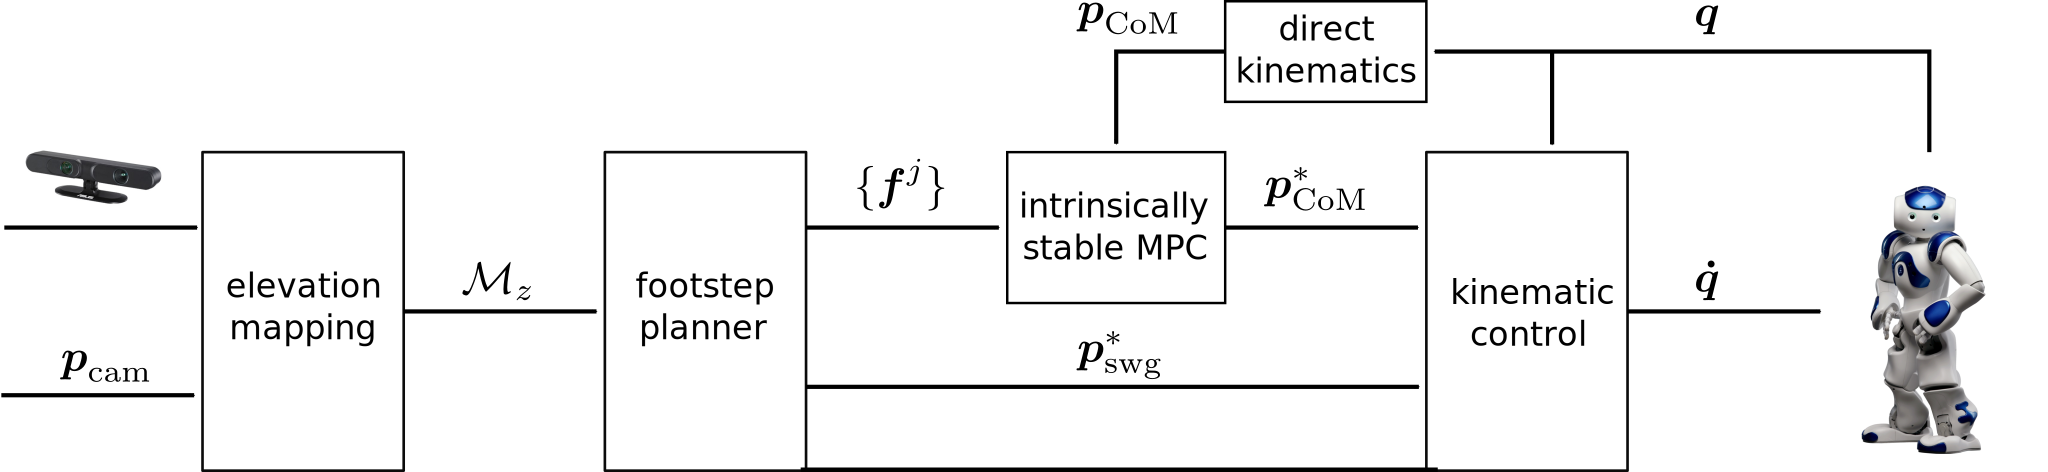
\includegraphics[width=\textwidth]{figures/BlockScheme.pdf}
  \caption{Block scheme of the approach.}
  \label{fig:block-scheme}
\end{figure}

This thesis extends \cite{ECC19}, providing an implementation of the
Variable-Height CoM IS-MPC for a real humanoid robot (NAO), extending the 
RRT-based footstep planner to work in a real environment with NAO and 
introducing \texttt{elevation\_mapping} (directly extending the block scheme
of \cite{ECC19}) in order to generate an elevation map of the terrain,
making NAO able to execute gaits in a \textit{World of Stairs} unknown
environment.

Chapter \ref{ch:elevation-map-generation} introduces
\texttt{elevation\_mapping}, describing the framework and its integration with
the camera, the planner and the robot. Chapter
\ref{ch:rrt-based-footstep-planning} describes the RRT-based footstep planner
introduced in \cite{ECC19}, formulating the problem and the algorithm and
discussing its integration with NAO. Chapter \ref{ch:vh-com-is-mpc} describes
the Variable-Height CoM IS-MPC and the implementation on the BHuman framework
\cite{BHumanCodeRelease2018}. Chapter \ref{ch:experiments} presents the
experiments performed on the robot in different scenarios, using the three
modules described in the previous three chapters. Chapter \ref{ch:conclusion}
concludes the thesis by summarizing the obtained results and discussing
future works.


\chapter{Elevation Map Generation}
\label{ch:elevation-map-generation}
When dealing with robot locomotion, the representation of the environment plays 
a fundamental role. It is, in fact, extremely important to properly
understand the structure of the world in order to safely make the robot move,
avoiding obstacles and dangerous zones, and to make it successfully complete 
its tasks. The world that surrounds the robot can be represented in many 
different ways; it is important to choose a proper representation to keep 
computational costs low and make to locomotion realizable.

In \textit{World of Stairs} scenarios, introduced in the previous chapter, the 
most efficient way to represent environments is by using elevation maps.
An elevation map is a grid that contains for each coordinate $(x, y)$ of the 
world its respective coordinate $z$. Hence, it can be seen as a function 
$\mathcal{M}_z$ such that, for each element $i$ of the grid,
$z_i = \mathcal{M}_z(x_i, y_i)$. This kind of representation allows the 
development of planners that quickly find plans to make robots move from a
position to another inside the world. 

This chapter introduces \texttt{elevation\_mapping}
\cite{Fankhauser2018ProbabilisticTerrainMapping}, the framework used in this 
thesis to generate elevation maps, which allow NAO to navigate in unknown 
environments (more precisely in \textit{World of Stairs} environments);
the ASUS Xtion Pro, an RGB-D sensor equipped on top of NAO, which has been 
used to send depth informaton to \texttt{elevation\_mapping}; 
the behaviour of the framework when a map is build using the ASUS Xtion Pro
placed on the head 
of NAO humanoid robot. The generated map is the one used in the experiment 
``Stair Climbing in Unknown Environment'', described in Section
\ref{sec:stair-climbing-unkenv}, and it is used by the footstep planner (Chapter
\ref{ch:rrt-based-footstep-planning}) to make NAO climb the stairs.

\section{Framework}
\texttt{elevation\_mapping} \cite{Fankhauser2018ProbabilisticTerrainMapping}
is a framework that allows to create elevation maps 
in rough environments using proprioceptive localization and distance sensors 
of the robot in real-time. The generated map is robot-centric,
meanining that the map is a local representation of the environment that 
surrounds the robot. Using a robot-centric representation instead of a 
world-centric one (where the map is expressed with respect to an inertial 
frame) has the advantage of not depending on the global pose of the robot.
This allows to avoid problems related to drift in the state estimation 
which would cause the maps 
to be inconsistent and not accurate enough to be used for locomotion.

The framework represents the map as a grid, providing for each cell a 
probabilistic distribution of the height of the terrain in the 
corresponding position. The map is updated using range measurements, provided 
by a sensor mounted on the robot, and the motion of the robot,
provided by a localization module such as a Kalman filter.
The program supports dynamic environments and it is built in C++, providing 
a ROS \cite{ros-melodic} interface which makes it simple to be integrated with
external sensors and other programs. \texttt{elevation\_mapping} is built 
upon GridMap \cite{Fankhauser2016GridMapLibrary}, which efficiently manages 
2D grid representations.

Even if not all the characteristics of the framework have been used in this 
thesis, the choice to integrate \texttt{elevation\_mapping} into the project 
has been essential to quickly build elevation maps that can be used by a
footstep planner (Chapter \ref{ch:rrt-based-footstep-planning}). Moreover, its 
versatility (because of the ROS interface) and its capabilities to generate 
efficiently maps for rough and dynamic environments, set a good starting point 
to extend this project to more complex scenarios. This section gives a brief 
overview of the framework without describing all the features in detail,
thoroughly described in \cite{Fankhauser2018ProbabilisticTerrainMapping}.

\subsection{Definitions}
The notation of the reference frames used by the framework are illustrated in 
Fig. \ref{fig:elevationmapping-coords-illustration}. In particular, $I$ is the 
inertial frame, $B$ is the base frame, $S$ is the sensor frame and $M$ is the 
map frame. The inertial frame $I$ is considered to be fixed with respect to the 
terrain. Both the base frame $B$ and the sensor frame $S$ are attached to the 
robot and it is assumed that the transformation $(r_{BS}, \Phi_{BS})$ between 
the two is known in advance. The elevation map is attacched to  
the reference frame $M$. $B$ and $M$ are related through a transformation 
$(r_{BM}, \Phi_{BM})$ given by the user. The $z$ axis of the map frame $M$ and 
the inertial frame $I$ are always aligned. A cell $i$ of the elevation map 
corresponding to the point of the surface $P_i = (x_i, y_i, \hat{h}_i)$,
which is expressed 
with respect to $M$. The transform $(r_{IB}, \Phi_{IB})$ between the position
of the robot $B$ and the 
inertial frame $I$ is provided by a state estimation module.
\begin{figure}
  \centering
  \includegraphics[width=\textwidth]
      {figures/elevationmapping-coords-illustration.png}
  \caption{The figure shows the notation of the reference frames used by 
      \texttt{elevation\_mapping}.
      \cite{Fankhauser2018ProbabilisticTerrainMapping} together with the 
      robot moving inside a rough environment.}
  \label{fig:elevationmapping-coords-illustration}
\end{figure}

\subsection{Map Update}
The map is updated when new measurements are read by the distance sensor and 
when the localization module updates the position of the robot. Each 
measurement $\tensor[_S]{r}{_{SP}}$ in the sensor frame $S$ is first transformed 
into the corresponding height measurement $p$ using the kinematic 
representation described before (Fig.
\ref{fig:elevationmapping-coords-illustration}).
The new height measurement can be represented as a Gaussian probability
distribution $\tilde{p} \sim \mathcal{N}(p, \sigma_p^2)$ given the sensor noise 
model \cite{Fankhauser2015Kinectv2}. In this way, it is possible to update 
the current estimate of the height $\mathcal{N}(\hat{h}, \sigma_h^2)$ by using 
a 1D Kalman filter, obtaining a new estimate of the height
$\mathcal{N}(\hat{h}^{+}, \sigma_h^{2+})$. The filter is updated only if the 
new measurement is not too far away (in terms of Mahalanobis distance)
from the current estimate.

The height estimate of each cell needs to be updated also during motion in 
order to take  
into account the uncertainty of the motion itself. To speed up the process,
each cell $i$ is extended with a spatial covariance matrix $\Sigma_{P_i}$ that,
in addition to the uncertainty of the height $\sigma_{h_i}^2$,
considers the uncertainty along the $x$ and $y$ axes.

\subsection{Map Fusion and Dynamic Environments}
The map fusion step is performed whenever required and it consists in 
transforming the elevation map data from a probabilistic representation of the 
kind $\mathcal{N}(\hat{h}_i, \Sigma_{P_i})$ to a deterministic representation 
$(\hat{h}_i, h_{i,\min}, h_{i,\max})$, where the values $h_{i,\min}, h_{i,\max}$
respectively represent the lower and the upper bound of the height estimation 
such that $h_i$ has 95\% probability of being in the range $[h_{i,\min},
h_{i,\max}]$. In this thesis the fused map is used by the footstep planner 
(Chapter \ref{ch:rrt-based-footstep-planning}) to generate a plan for the robot,
similarly to \cite{Fankauser2018RobustRoughTerrainLocomotion}.

\texttt{elevation\_mapping} handles dynamic environments by performing a 
visibility check based on ray tracing. Since this is a computationally 
expensive task, it is performed in parallel to the data acquisition process and 
it is run at a low frequency~(1 Hz).

\section{ASUS Xtion Pro}
The camera (Fig. \ref{fig:asus-xtion-pro}) used in this thesis is an
ASUS Xtion Pro \cite{ASUSXtionProWebsite},
which is equipped with a depth sensor, used to generate the height measurements
sent to \texttt{elevation\_mapping}. The communication between the camera and 
the mapping framework is handled by ROS.
ASUS Xtion Pro works up to a resolution of $640\times480$
at 30 fps. Its working range is from 0.5m up to 3.5m. The camera has been 
calibrated with a tool called \texttt{camera\_calibration}
\cite{cameracalibrationros}.
\begin{figure}
  \centering
  \includegraphics[width=0.5\textwidth]{figures/asus-xtion-pro.jpeg}
  \caption{The ASUS Xtion Pro \cite{ASUSXtionProWebsite} is equipped with a
      depth sensor and it is 
      easily configurable to make it work with ROS. This simplifies the 
      integration with \texttt{elevation\_mapping} and, consequently, 
      the construction of a navigable map.}
  \label{fig:asus-xtion-pro}
\end{figure}

\section{World of Stairs}
The integration between \texttt{elevation\_mapping} and the ASUS Xtion Pro 
allows to easily generate elevation maps in rough environments, meaning that 
the same settings could be used to generate elevation maps for \textit{World 
of Stairs} scenarios, described in the previous chapter.

As mentioned before, ROS simplifies the communication between the camera and 
the mapping framework, allowing to develop a block scheme (Fig.
\ref{fig:block-scheme}) that connects the camera to the robot. The humanoid 
robot used in this thesis is NAO, shown in Fig. \ref{fig:nao-with-xtion}
where it has been equipped with the ASUS Xtion Pro.

The \textit{World of Stairs} scenario considered for the experiments is the one 
shown in Fig. \ref{fig:nao-with-xtion-full-env}, where the robot stands in 
front of a stairway. The idea is to position the camera towards the stairs in 
order to generate an elevation map accurate enough to be used by a footstep
planner (Chapter \ref{ch:rrt-based-footstep-planning}). Given the pose of the 
camera, which is sent to \texttt{elevation\_mapping} together with the depth 
information of the camera, it is possible to quickly generate a map.
Of course, the area underneath the robot can not be seen by the camera. That is 
why a ``safe zone'' is manually added to the final elevation map before 
sending it to the planner.
Fig. \ref{fig:onlymap-xtion-20cm} shows the map generated by the framework 
(together with the ``safe zone'') when the 
camera is oriented towards the stairs (as in Fig. \ref{fig:xtion-rgb-20cm}).
The generated map is the one used by the footstep planner in the scenario 
``Stair Climbing in Unknown Environment'', described in Section
\ref{sec:stair-climbing-unkenv}, where NAO is able to climb the stairs in an 
unknown environment.
\begin{figure}
  \begin{subfigure}[b]{0.49\textwidth}
    \includegraphics[width=\textwidth]{figures/NAO-with-xtion.JPEG}
    \caption{}
    \label{fig:nao-with-xtion}
  \end{subfigure}
  \hfill
  \begin{subfigure}[b]{0.49\textwidth}
    \includegraphics[width=\textwidth]{figures/NAO-with-xtion-full-env.JPEG}
    \caption{}
    \label{fig:nao-with-xtion-full-env}
  \end{subfigure}
  \caption{On the left, NAO humanoid robot with ASUS Xtion Pro placed on top.
      On the right, NAO humanoid robot in the environment described TODO, 
      right before starting the execution of the experiment.}
\end{figure}
\begin{figure}
  \centering
  \includegraphics[width=0.85\textwidth]{figures/xtion_rgb_20cm.png}
  \caption{RGB image seen by the ASUS Xtion Pro placed on top of the robot.
      The corresponding depth image is sent to \texttt{elevation\_mapping}
      to build the map.}
  \label{fig:xtion-rgb-20cm}
\end{figure}
\begin{figure}
  \centering
  \includegraphics[width=\textwidth]{figures/onlymap-xtion-20cm.pdf}
  \caption{Elevation map build by \texttt{elevation\_mapping} for the scenario 
      ``Stair Climbing in Unknown Environment'' described in section 
      \ref{sec:stair-climbing-unkenv}.}
  \label{fig:onlymap-xtion-20cm}
\end{figure}


\chapter{RRT-based Footstep Planning}
Generating plan considering NAO hparams.

Algorithms etc.


\chapter{Variable Height CoM IS-MPC}
LIP, variable height CoM. MPC (BHuman implementation). Cite
\cite{SYROCO18}.

\section{LIP}
Where it comes from, proofs and prev. works.

3D CoM dynamics.

Moment balance around ZMP for the $x$ coordinate:
\begin{equation}
  (z_c - z_z) \ddot{x}_c = (\ddot{z}_c + g) (x_c + x_z)
\end{equation}
where $g$ is the gravity acceleration. Identical for $y$. Dynamics of $x$, $y$
coordinates of the CoM:
\begin{align}
  \ddot{x}_c &= \frac{\ddot{z}_c + g}{z_c - z_z} (x_c - x_z) \\
  \ddot{y}_c &= \frac{\ddot{z}_c + g}{z_c - z_z} (y_c - y_z)
\end{align}
Force balance along $z$ axis leads to structurally different dynamics for the 
corresponding coordinate:
\begin{equation}
  \ddot{z}_c = \frac{f_z}{m} - g
\end{equation}
where $f_z$ denotes the z-component of the ground reaction force (GRF), acting 
as an external input, and $m$ is the total mass of the humanoid.
SEE KAJITA HERE.

Condition for maintaining balance is that CoP is internal to SP. Since CoP, CoM,
ZMP are colinear, the condition is equivalent to the ZMP being internal to the 
polyhedral cone having CoM as vertex and SP as cross-section (Fig. 2 SYROCO18).

3D Linear Model (const height CoM) SECTION:

MAYBE MERGE THIS SECTION WITH THE PREV USING THEORY FROM KAJITA?

3D motion model of prev. section nonlinear, difficult to use for gait
generation. Usual way to make the model linear is to assume ground fully 
horizontal and CoM over the ground const, as a consequence $z_z = 0$, hence 
ZMP coincident with CoP. \textbf{LIP}:
\begin{align}
  \ddot{x}_c &= \omega_0^2 (x_c - x_z) \\
  \ddot{y}_c &= \omega_0^2 (y_c - y_z)
\end{align}
where $\omega_0^2 = g/\bar{z}_c$. 2D LINEAR MODEL NOT APPROPRIATE FOR GAIT
GENERATION OVER UNEVEN TERRAIN.

\section{3D Linear Model (variable height CoM)}

However, requiring CoM move at const height is not the only way to make the 
system linear. A more general way is to constraint its vertical motion so that:
\begin{equation}
  \frac{\ddot{z}_c + g}{z_c - z_z} = \omega^2
\end{equation}
with $\omega$ arbitrary const. LIP model can be seen as a particular case in
which $\omega^2 = \omega_0^2$. Using the above, eqs. CoM dynamics become:
\begin{align}
  \ddot{x}_c &= \omega^2 (x_c - x_z) \\
  \ddot{y}_c &= \omega^2 (y_c - y_z)
\end{align}
whereas the dynamics of $z_c$ is directly derived from the constraint itself:
\begin{equation}
  \ddot{z}_c = \omega^2 (z_c - z_z) - g
\end{equation}

The above dynamic equations are linear and have a clear LIP structure with 
ZMP coordinates $(x_z, y_z, z_z)$ acting as control inputs. THIS 3D MODEL 
ALLOWS VERTICAL MOTION OF THE COM AND THEREFORE CAN BE USED FOR GAIT GENERATION 
ON UNEVEN TERRAIN, IN CONJUNCTION WITH THE BALANCE CONDITION ILLUSTRATED IN 
FIG. 2 (SYROCO18).

DOUBLE CHECK NOTES ON SYROCO18 SEC. 2.2 PAGE 395.

\section{MPC Formulation + Algorithm}
Proofs as in report.pdf in order to easily introduce QP problem.

Assuming footstep sequence in given in advance: MPC scheme based on 3D model 
introduce above. Eqs. include an unstable subsystem, taken care by adding
stability constraint. Extends IS-MPC Scianca
\cite{DBLP:conf/humanoids/SciancaCSLO16}.

3.1. Motion Model

Dynamic extension: choose control variable as ZMP velocity $\dot{x}_z$ instead
of ZMP itself. On the x axis:
\begin{equation}
  \begin{pmatrix}
    \dot{x}_c \\
    \ddot{x}_c \\
    \dot{x}_z
  \end{pmatrix}
  =
  \begin{pmatrix}
    0 & 1 & 0 \\
    \omega^2 & 0 & -\omega^2 \\
    0 & 0 & 0
  \end{pmatrix}
  \begin{pmatrix}
    x_c \\
    \dot{x}_c \\
    x_z
  \end{pmatrix}
  +
  \begin{pmatrix}
    0 \\
    0 \\
    1
  \end{pmatrix}
  \dot{x}_z
\end{equation}
Dynamics are the same along three axes with additive term along z axis.

Using piecewise-constant control inputs over sampling intervals of duration 
$\delta$, with a prediction horizon $T_h = N \dot \delta$. Current time instant
$t_k$, successive instants within prediction horizon $t_k+i, i = 1, \dots, N$.
Similar notation for other variables. At a generic isntant $t_j$:
\begin{equation}
  \dot{x}_z(t) = \dot{x}_z^j, t \in [t_j, t_{j+1})
\end{equation}
so that the ZMP x-position in the time interval $[t_j, t_{j+1}]$ is:
\begin{equation}
  x_z(t) = x_z^j + (t - t_j) \dot{x}_z^j, t \in [t_j, t_{j+1}]
\end{equation}

3.2. ZMP constraints

2D case first. ZMP inside the SP. $(x_f^j, y_f^j, \theta_f^j)$ pose of the 
generic footstep within assigned sequence. Fixed-shape moving ZMP constraint to
enforce balance. Admissible region for ZMP at $t_{k+i}$ is centered in 
$(x_f^{k+i}, y_f^{k+i})$ and has orientation $\theta_f^{k+i}$.

SS: $(x_f^{k+i}, y_f^{k+i}, \theta_f^{k+i})$ coincide with the pose of the 
support foot, hence, $(x_f^j, y_f^j, \theta_f^j)$.

DS: $(x_f^{k+i}, y_f^{k+i}, \theta_f^{k+i})$ gradually slide from the position 
and orientation of the previous support foot to those of the next. [NOT 
STRICTLY NECESSARY, DOUBLE CHECK IN IMPLEMENTATION AS WELL].

ZMP constraint in 2D:
\begin{equation}
  \label{eq:zmp-constraint-2d}
  -\frac{1}{2}
  \begin{pmatrix}
    d_x^\text{z} \\
    d_y^\text{z}
  \end{pmatrix}
  \le
  R_{k+i}^T
  \begin{pmatrix}
    x_z^{k+i} - x_f^{k+i} \\
    y_z^{k+i} - y_f^{k+i}
  \end{pmatrix}
  \le
  \frac{1}{2}
  \begin{pmatrix}
    d_x^\text{z} \\
    d_y^\text{z}
  \end{pmatrix}
\end{equation}
where $d_x^\text{z}$ and $d_y^\text{z}$ are the dimensions of the rectangular
constraint region and $R_{k+i}^T$ is the rotation matrix associated with
$\theta_f^{k+i}$. Note that $(x_z^{k+i}, y_z^{k+i})$ is the predicted position
of the ZMP, which can be expressed as a linear combination of the control
variables:
\begin{equation}
  \label{eq:piecewise-linear-zmp-trajectory}
  x_z^{k+i} = x_z^k + \delta \sum_{i=0}^{i-1} \dot{x}_z^{k+j}
\end{equation}
Eq. \eqref{eq:zmp-constraint-2d} must be imposed for $i = 1, \dots, N$.

ZMP constraint in 3D:
ZMP is allowed to leave the ground in order to generate vertical CoM motions,
balance condition now requires ZMP to remain inside polyhedral cone defined 
by SP and CoM. When ZMP is allowed to move vertically, the cone defines a 
nonlinear constraint. In order to remove nonlinearity, box constraint:
\begin{equation}
  \label{eq:zmp-constraint-3d}
  -\frac{1}{2}
  \begin{pmatrix}
    \tilde{d}_x^\text{z} \\
    \tilde{d}_y^\text{z} \\
    d_z^\text{z}
  \end{pmatrix}
  \le
  R_{k+i}^T
  \begin{pmatrix}
    x_z^{k+i} - x_f^{k+i} \\
    y_z^{k+i} - y_f^{k+i} \\
    z_z^{k+i} - y_f^{k+i}
  \end{pmatrix}
  \le
  \frac{1}{2}
  \begin{pmatrix}
    \tilde{d}_x^\text{z} \\
    \tilde{d}_y^\text{z} \\
    d_z^\text{z}
  \end{pmatrix}
\end{equation}
where $d_z^\text{z}$ defines the maximum allowed vertical ZMP displacement
w.r.t. the horizontal patch. To guarantee that the box is consteind in the cone:
\begin{equation}
  \tilde{d}_x^\text{z} = d_x^\text{z} \left( 1 -
      \frac{d_z^\text{z}}{2z_c^{\min}} \right)
      - \frac{d_z^\text{z}}{z_c^{\min}}\Delta x_c
\end{equation}
where $\Delta x_c$ max expected displacement of CoM w.r.t. center of support 
foot and $z_c^{\min}$ is the minimum expected value for CoM height.
Analogous for $\tilde{d}_y^\text{z}$.

Similarly to 2D case, box constraint kept fixed during SS. During DS box 
slide linearly from its position around the previous support foot to its 
position around the next support foot, thus, always remaining within the 
polyhedral cone which defines the ZMP balance constraint (Fig. 5 SYROCO18).

3.3. Stability constraint

Motion model unstable, generic solution diverges making components of CoM 
unbounded w.r.t. ZMP position, generated gait infeasible.
In \cite{DBLP:conf/humanoids/SciancaCSLO16} it was shown (TODO: report proof 
here) that if the initial condition $(x_c^k, \dot{x}_c^k)$ satisfies:
\begin{equation}
  \label{eq:stability-condition-xc}
  x_c^k + \frac{\dot{x}_c^k}{\omega} = \omega \int_{t_k}^\infty 
      e^{-\omega(\tau-t_k)}x_z(\tau)d\tau
\end{equation}
then the solution of $x_c$ dynamics (TODO: eqref) remains bounded for all
$t$. Similar for $y_c$ dynamics. Regarding $z_c$:
\begin{equation}
  \label{eq:stability-condition-zc}
  z_c^k + \frac{\dot{z}_c^k}{\omega} = \frac{g}{\omega^2} +
      \omega \int_{t_k}^\infty e^{\omega(\tau-t_k)}z_z(\tau)d\tau
\end{equation}

MPC formulation, stability condition \eqref{eq:stability-condition-xc} can be 
enforced by writing it as a constraint on the control variables
$\dot{x}_z^{k+i}$:
\begin{equation}
  \label{eq:stability-constraint-xdot}
  \frac{1}{\omega}\frac{1-e^{-\delta\omega}}{1-e^{-N\delta\omega}}
    \sum_{i=0}^{N-1} e^{-i\delta\omega} \dot{x}_z^{k+i} =
    x_c^k + \frac{\dot{x}_c^k}{\omega} - x_z^k
\end{equation}
(using integral eqref{eq:stability-condition-xc} + piecewise linear ZMP trajectory
\eqref{eq:piecewise-linear-zmp-trajectory} + infinite replication). TODO:
infinite replication proof here.

Stability constraint on $z_c$ derived from \eqref{eq:stability-condition-zc}:
\begin{equation}
  \label{eq:stability-constraint-zdot}
  \frac{1-e^{-\delta\omega}}{1-e^{-N\delta\omega}}
    \sum_{i=0}^{N-1} e^{-i\delta\omega} \dot{z}_z^{k+i} =
    z_c^k + \frac{\dot{z}_c^k}{\omega} - z_z^k - \frac{g}{\omega^2}
\end{equation}
where $\dot{z}_z$ is set to zero beyond prediction horizon (TODO: proof here).

4. MPC Algorithm

MPC algorithm which solves QP problem at each iteration.

4.1, Formulation of the QP problem

Defining the decision variables vectors:
\begin{align}
  \dot{X}_\text{z}^k&=(\dot{x}_\text{z}^k, \dots, \dot{x}_\text{z}^{k+N-1})^T \\
  \dot{Y}_\text{z}^k&=(\dot{y}_\text{z}^k, \dots, \dot{y}_\text{z}^{k+N-1})^T \\
  \dot{Z}_\text{z}^k&=(\dot{z}_\text{z}^k, \dots, \dot{z}_\text{z}^{k+N-1})^T
\end{align}
QP problem:
\begin{align*}
  \min_{\dot{X}_\text{z}^k, \dot{Y}_\text{z}^k, \dot{Z}_\text{z}^k}
      &\sum_{i=1}^N
      \biggl[
          (\dot{x}_z^{k+i})^2 +
          (\dot{y}_z^{k+i})^2 +
          (\dot{z}_z^{k+i})^2 + \\
          &\beta \biggl(
              (x_z^{k+i} - x_f^{k+i})^2 +
              (y_z^{k+i} - y_f^{k+i})^2 +
              (z_z^{k+i} - z_f^{k+i})^2
          \biggr)
      \biggr]\\
      \textrm{s.t. } &\textrm{ZMP constraint \eqref{eq:zmp-constraint-3d}} \\
      &\textrm{stability constraints \eqref{eq:stability-constraint-xdot},
          \eqref{eq:stability-constraint-zdot}}
\end{align*}
where the cost function includes the decision variables for regularization 
purposes and a term which attempts to bring the ZMP to patch level whenever 
possible (TODO: actually to center of the footstep).

4.2. Algorithm

Todo.

\section{BHuman implementation}
BHuman + NAO.

\section{Conclusion}
Conclude by summarizing importance of the model + simulations in
separate ch.


\chapter{Experiments}
\label{ch:experiments}

To test the behaviour of the whole project, multiple experiments have been 
performed. In particular, different scenario and test cases have been designed 
in order to study in detail the functionalities of the robot and each program.
As previously introduced, the humanoid robot used for the experiments of this 
thesis is NAO \cite{NAOdesign}, which has been equipped with an ASUS Xtion 
Pro RGB-D camera \cite{ASUSXtionProWebsite}, placed on top of its head.
As mentioned in the first chapter, the camera communicates with
\texttt{elevation\_mapping} (Chapter \ref{ch:elevation-map-generation}),
which creates a representation of the environment
called elevation map, which is used by the footstep planner, described in 
Chapter \ref{ch:rrt-based-footstep-planning}, to generate a safe and feasible 
plan for the robot. The footsteps are sent to the robot, which runs an 
implementation of the Variable Height CoM Intrinsically Stable MPC (Chapter 
\ref{ch:vh-com-is-mpc}) that allows the robot to correctly performe the 
desired motion, making it navigate in a \textit{World 
of Stairs} environment.

The experiments have been performed by initially checking the real capabilities 
of the robot, making it first climb a single staircase and then a stairway 
composed of multiple staircases, in order to better understand 
the kind of scenario that NAO can handle. At this point only the MPC is 
used, assigning the footsteps manually. Then, the footstep planner is 
introduced into the project, making NAO navigate autonomously from its initial 
position to a goal region, given an elevation map of the environment which has 
been manually created. In the end, NAO is equipped with an ASUS Xtion Pro 
camera. This allows to introduce \texttt{elevation\_mapping} to the project,
generating autonomously elevation maps, making NAO able to move in 
a \textit{World of Stairs} environment which is not known a priori,
correctly climbing the stairs in order to reach a desired position.

\section{NAO and Computer Settings}
The NAO v5 humanoid robot (Fig: \ref{fig:nao-with-xtion-2}), developed by 
Softbank, is 57 cm tall and weights 5.4 kg. It is equipped with an Intel ATOM 
Z530 processor which has a frequencly of 1.6 Ghz, 1 GB of RAM and 2 GB of 
flash storage. It has 25 DoF, 7 touch sensors located on the head, the hands 
and the feet, two internal cameras, 4 microphones, a speaker, sonar and IMU 
sensors. The framework used for the experiments, which has been installed on 
the robot, is BHuman \cite{BHumanCodeRelease2018}, which simplifies the 
development of on board algorithms by organizing the framework in modules.
When using the full settings, NAO is equipped with an ASUS Xtion Pro RGB-D
camera,
which is connected to an external computer via a USB cable. This external 
computer communicates with NAO via an ethernet cable through TCP.
Both \texttt{elevation\_mapping} and the footstep planner run on the external 
computer, which is equipped with an Intel Core i5-5257U with 2.70 GHz
base frequency and 16 GB of RAM. The Variable Height CoM IS-MPC runs on the 
robot. 
\begin{figure}
  \centering
  \includegraphics[width=0.5\textwidth]{figures/NAO-with-xtion-2.JPEG}
  \caption{The figure shows NAO v5 humanoid robot, the platform
      used for the experiments of this thesis, equipped with an ASUS Xtion
      Pro RGB-D camera. The camera is connected via USB to an external 
      computer which runs \texttt{elevation\_mapping} and the footstep 
      planner. The external computer communicates with NAO through an 
      ethernet cable using TCP.}
  \label{fig:nao-with-xtion-2}
\end{figure}


\section{Simple Staircase}
Staircase from 1cm to 5cm. Limitations of the robot.
\begin{figure}
  \centering
  \includegraphics[width=\textwidth]
      {figures/experiments/simple-staircase/xy-plot-4cm.pdf}
  \includegraphics[width=\textwidth]
      {figures/experiments/simple-staircase/xz-plot-4cm.pdf}
  \caption{The plots show how the CoM and the ZMP vary with respect to the
		footsteps in the scenario ``Simple Staircase''.
    The green boxes represent the footsteps.}
  \label{fig:experiments:simple-staircase:comzmp}
\end{figure}

\section{Multiple Staircases}
Two consecutive staircases of 2cm.

\subsection{Upstairs}
Upstairs.
\begin{figure}
  \begin{subfigure}{0.48\textwidth}
    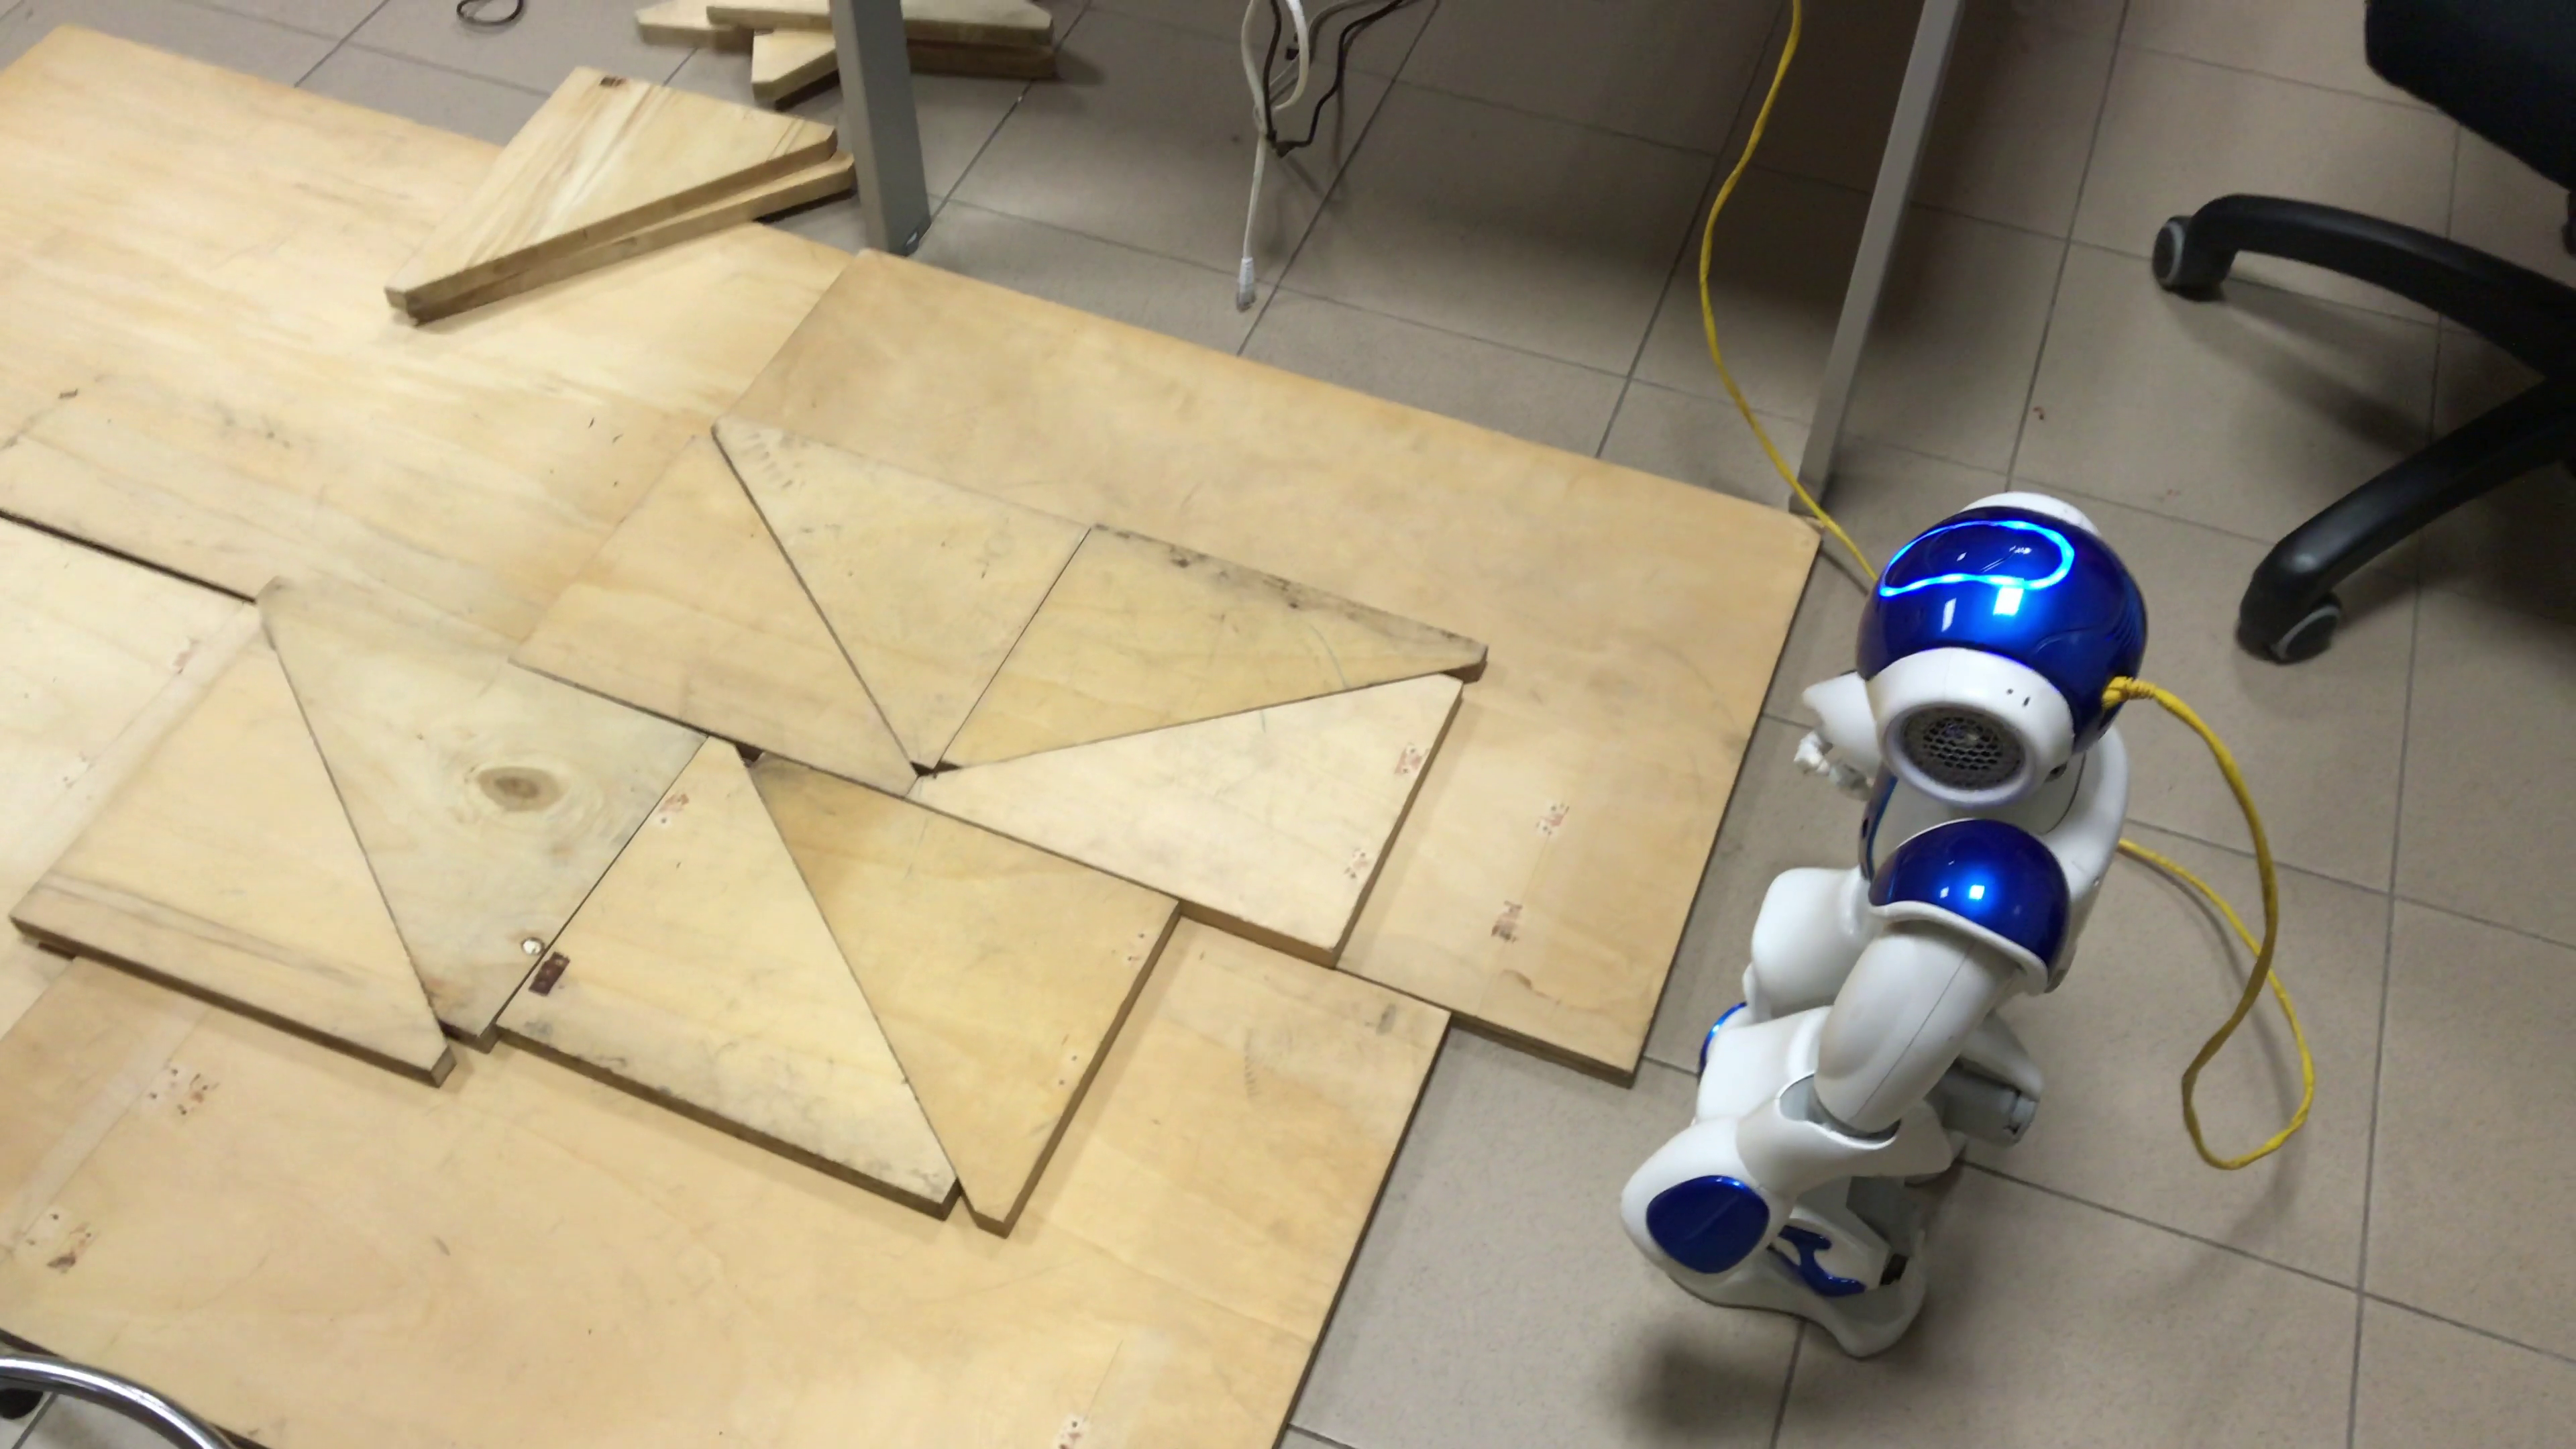
\includegraphics[width=\linewidth]
      {figures/experiments/multiple-staircases/upstairs/video/01.png}
    \caption{Starting position}
    \label{fig:exp:ms:up:frame1}
  \end{subfigure}\hspace*{\fill}
  \begin{subfigure}{0.48\textwidth}
    \includegraphics[width=\linewidth]
      {figures/experiments/multiple-staircases/upstairs/video/02.png}
    \caption{First step}
  \end{subfigure}
  \begin{subfigure}{0.48\textwidth}
    \includegraphics[width=\linewidth]
      {figures/experiments/multiple-staircases/upstairs/video/03.png}
    \caption{Second step}
  \end{subfigure}\hspace*{\fill}
  \begin{subfigure}{0.48\textwidth}
    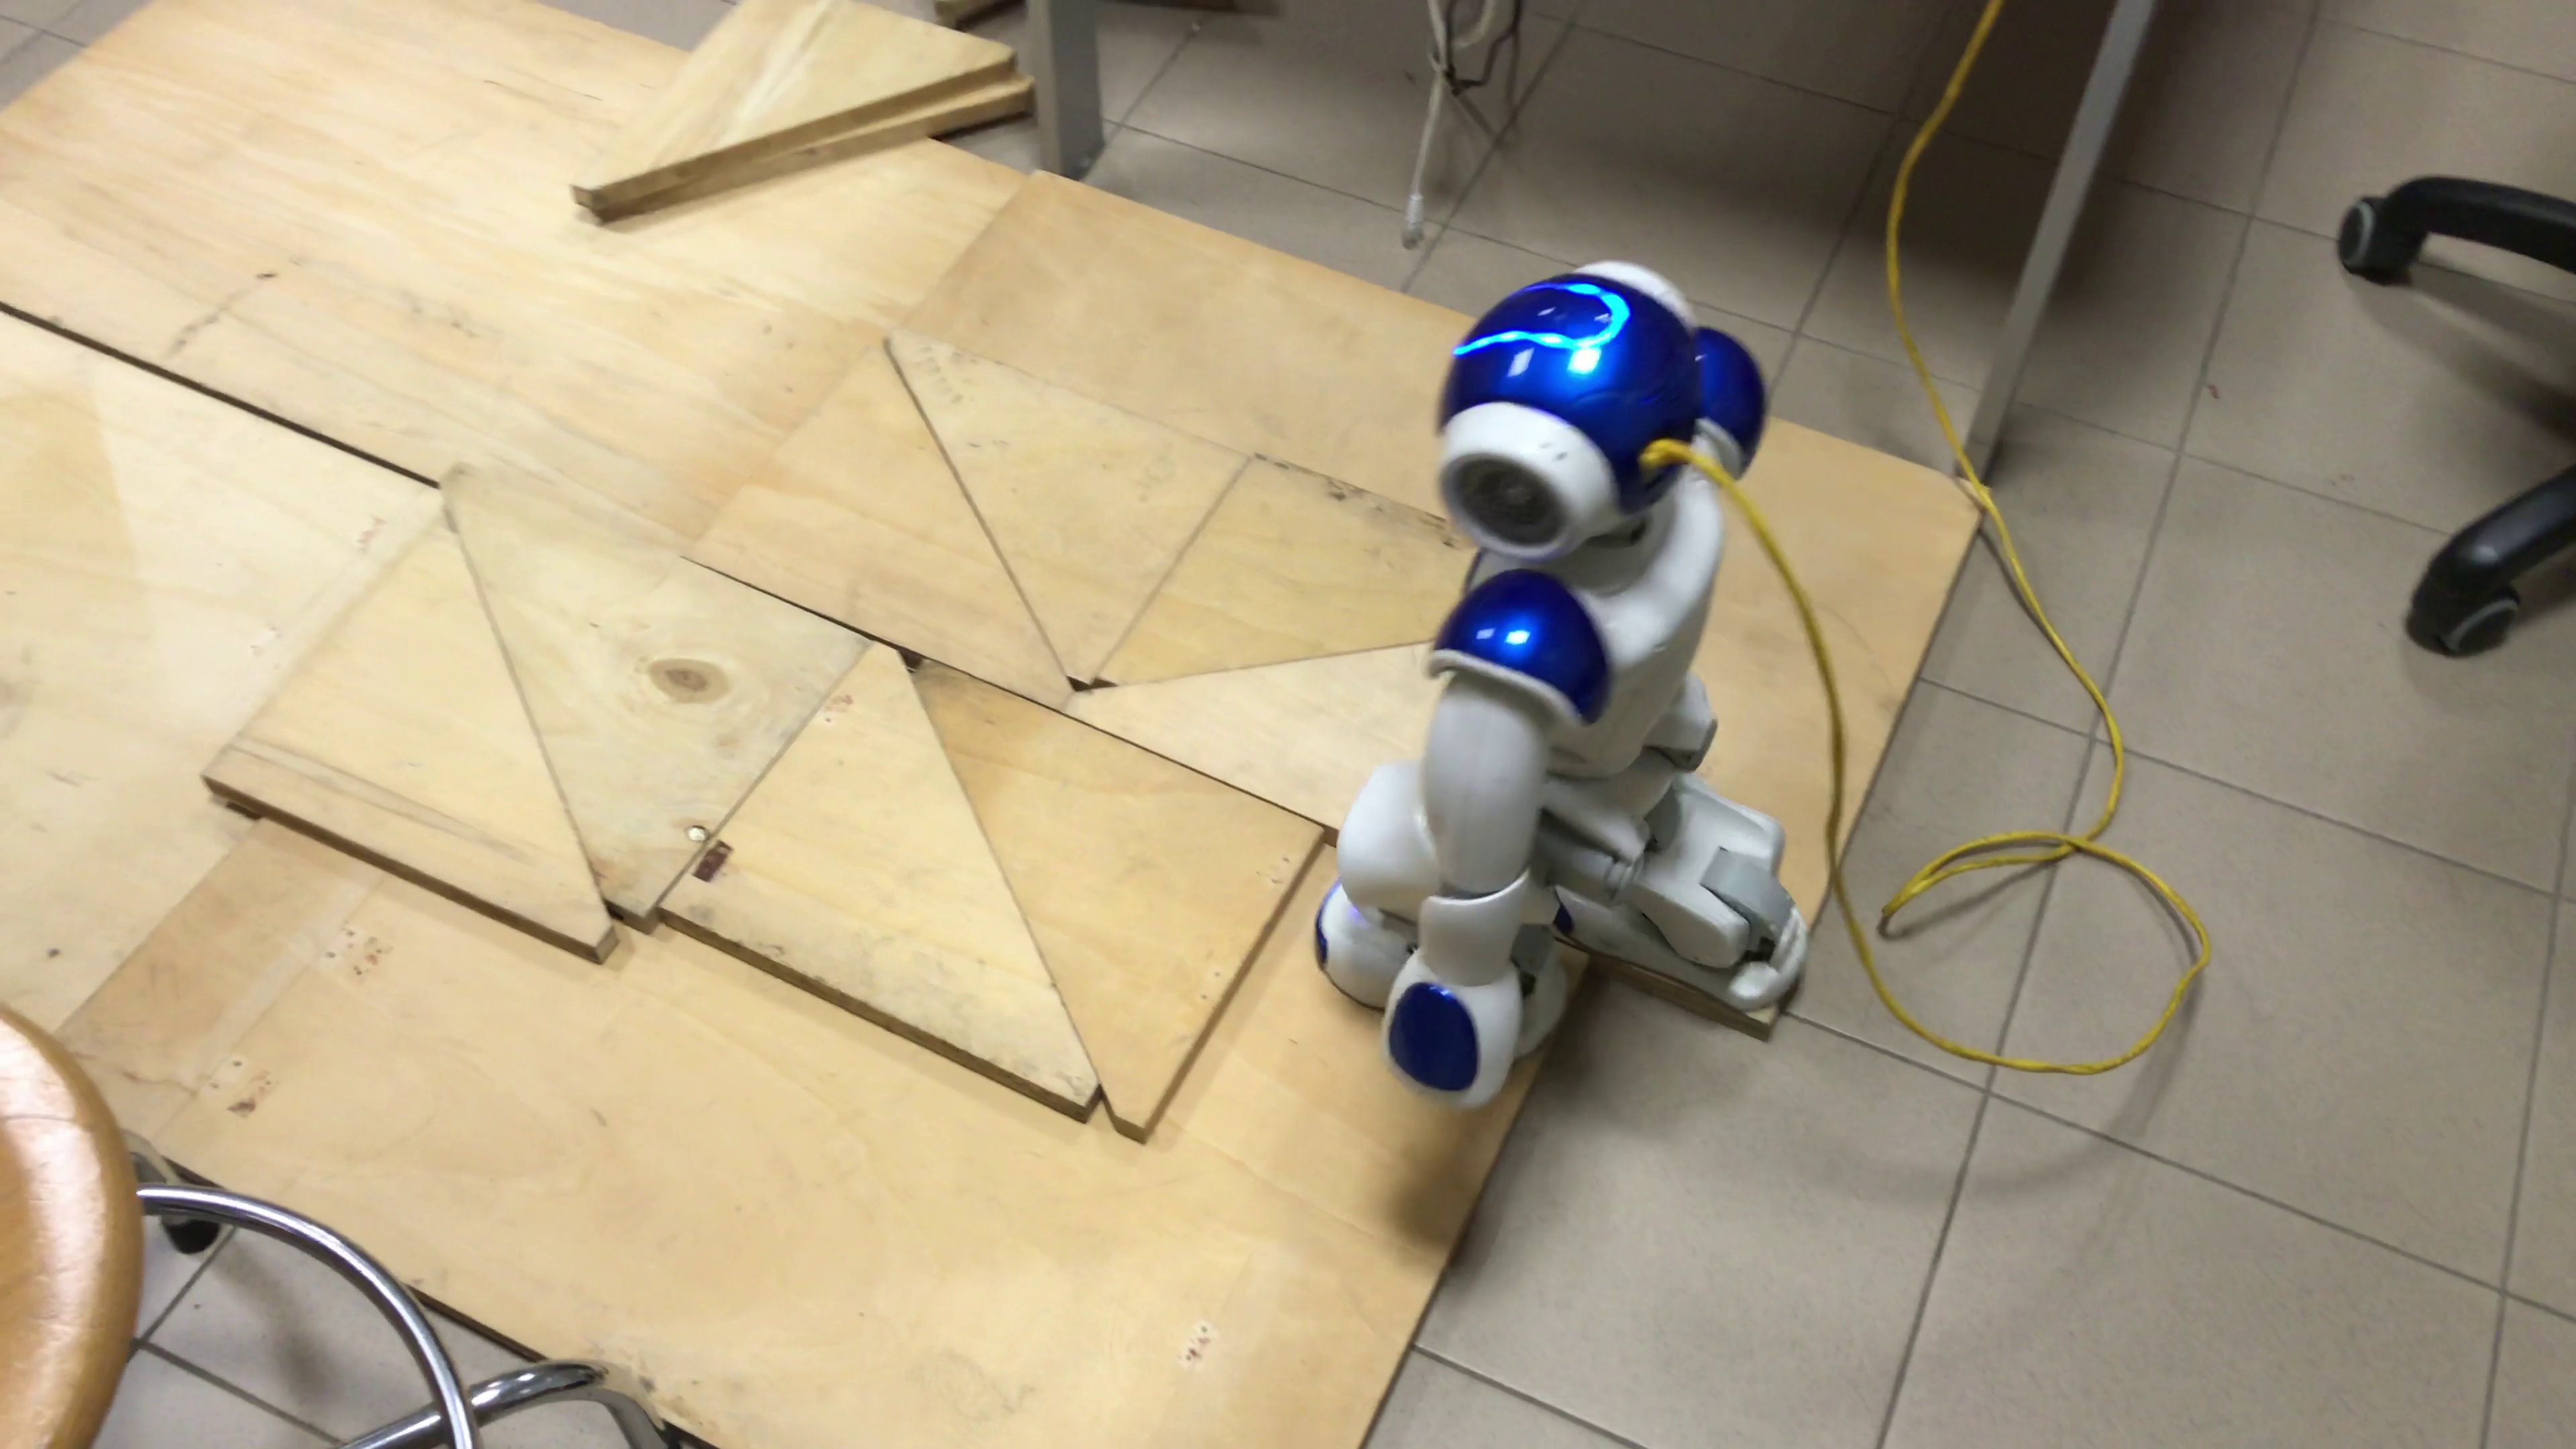
\includegraphics[width=\linewidth]
      {figures/experiments/multiple-staircases/upstairs/video/04.png}
    \caption{Third step}
  \end{subfigure}
  \begin{subfigure}{0.48\textwidth}
    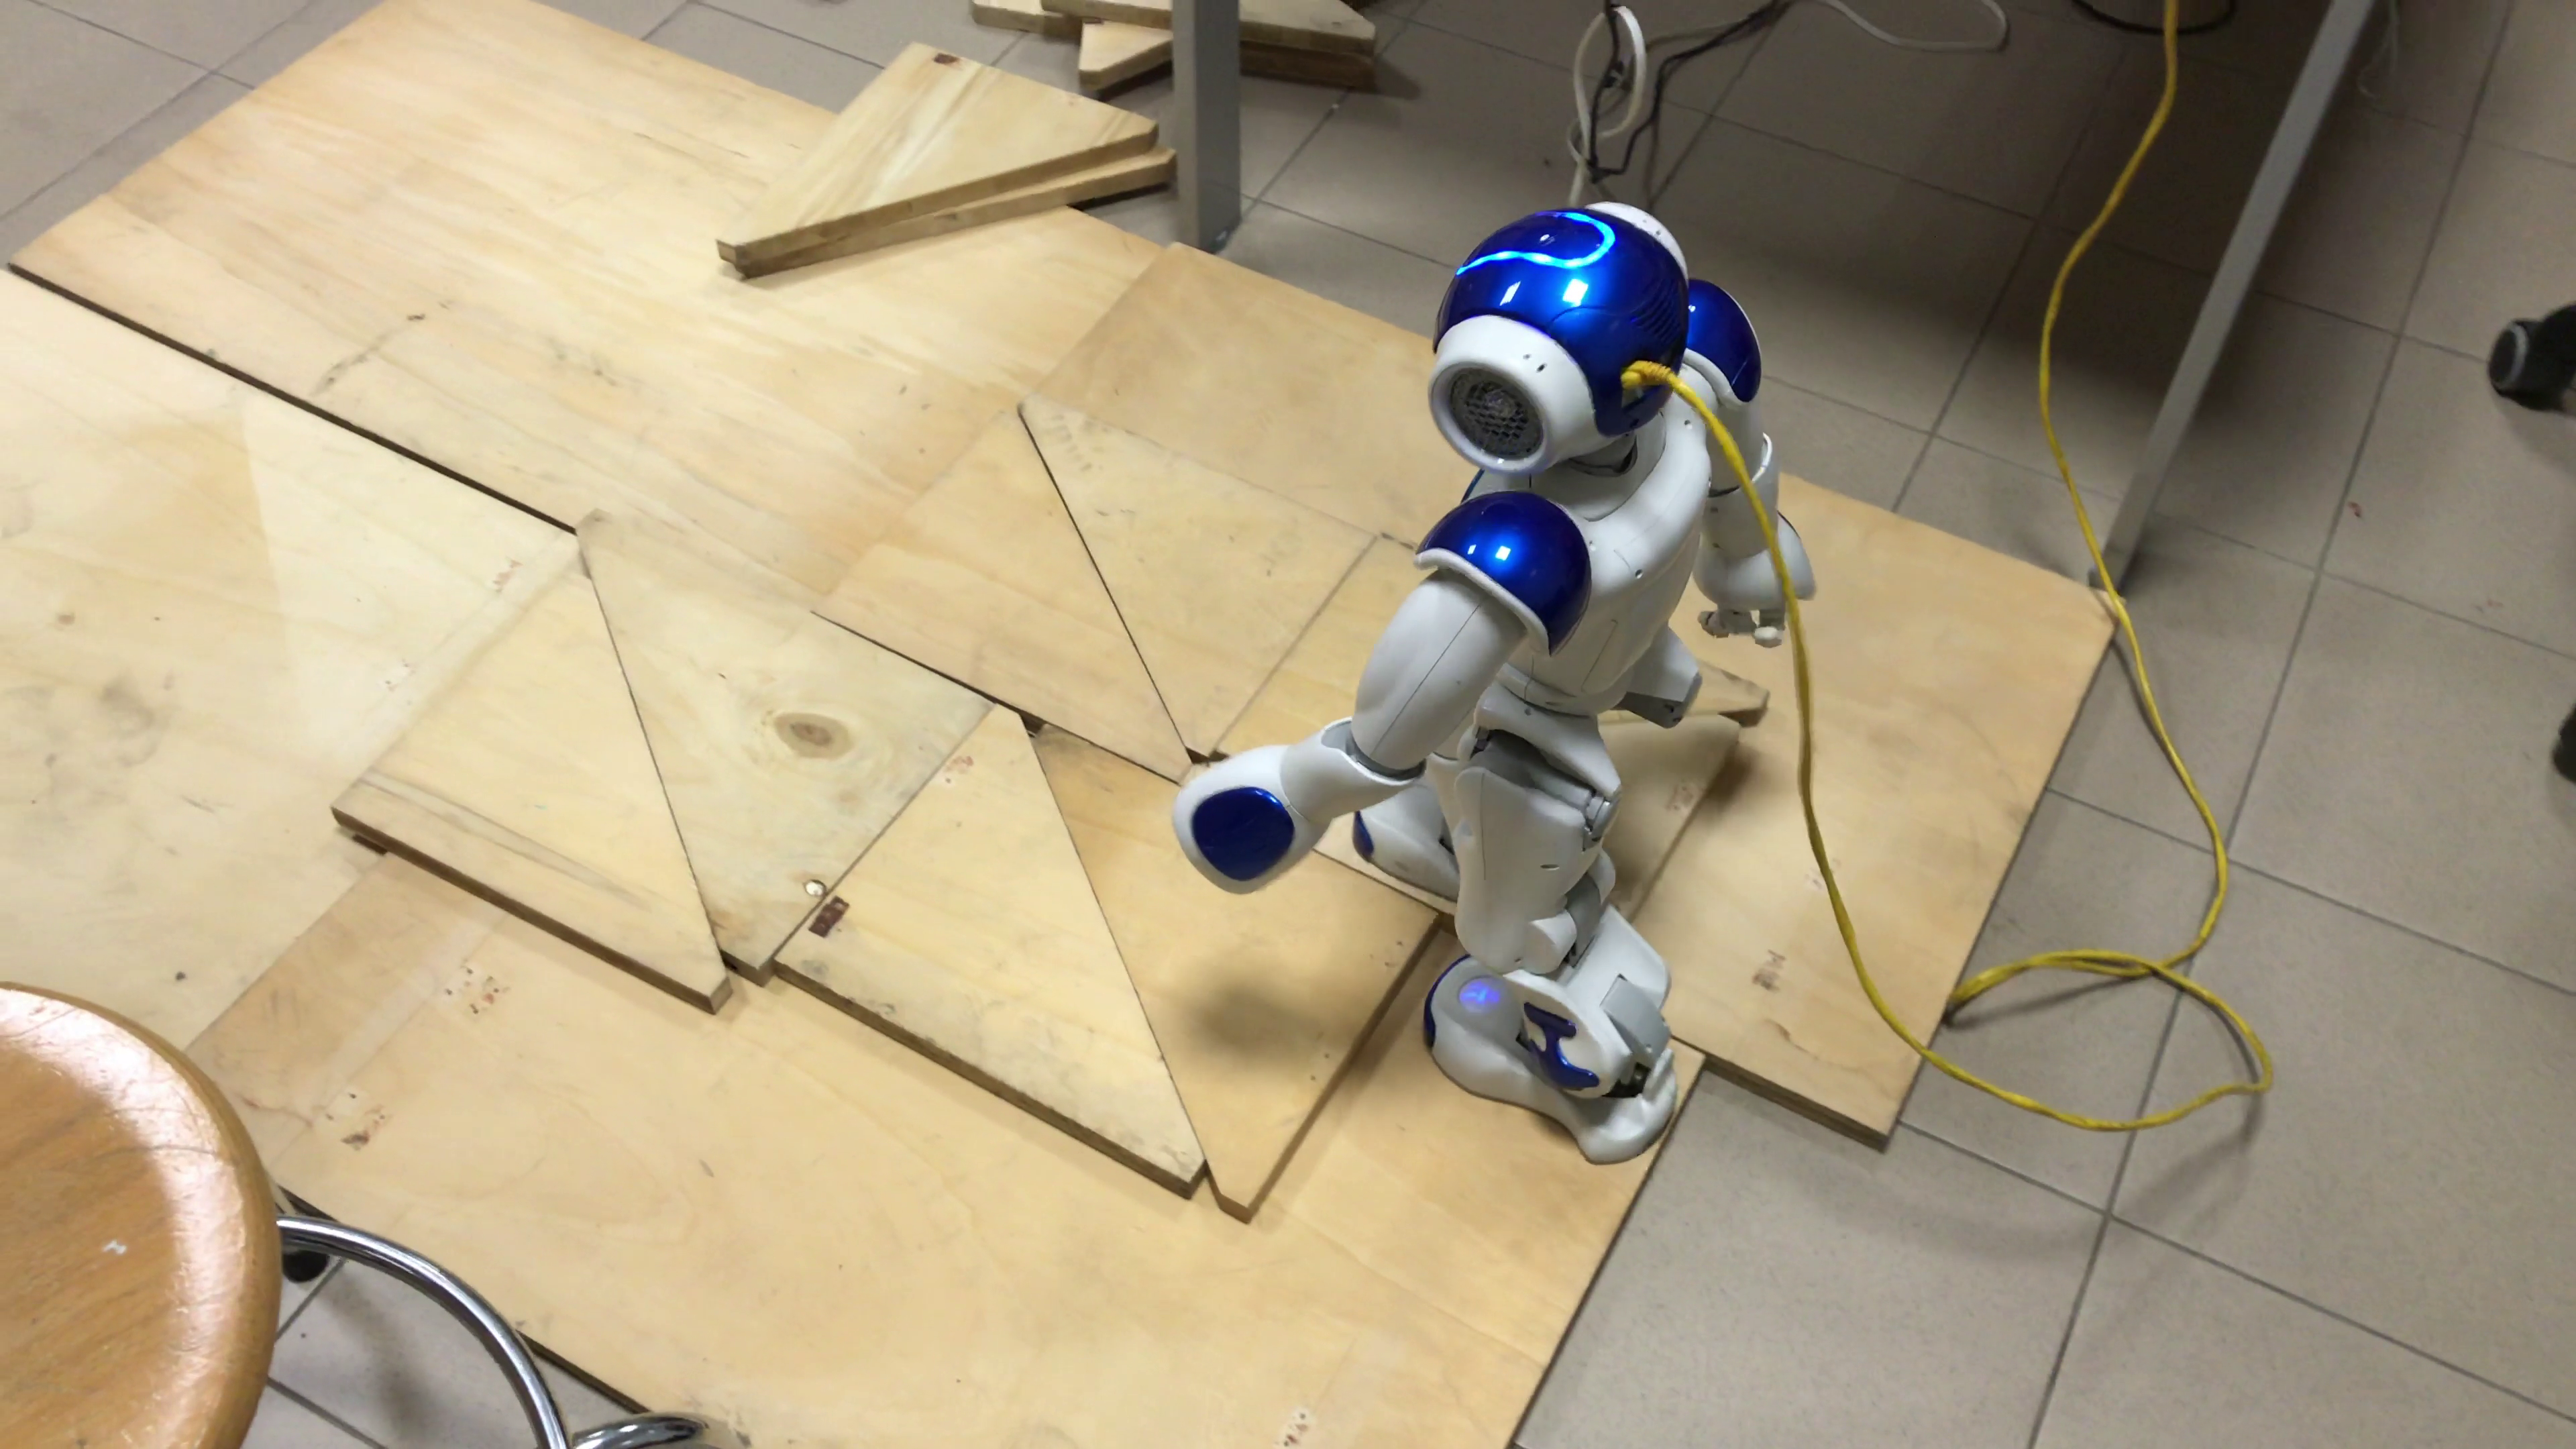
\includegraphics[width=\linewidth]
      {figures/experiments/multiple-staircases/upstairs/video/05.png}
    \caption{Fourth step}
  \end{subfigure}\hspace*{\fill}
  \begin{subfigure}{0.48\textwidth}
    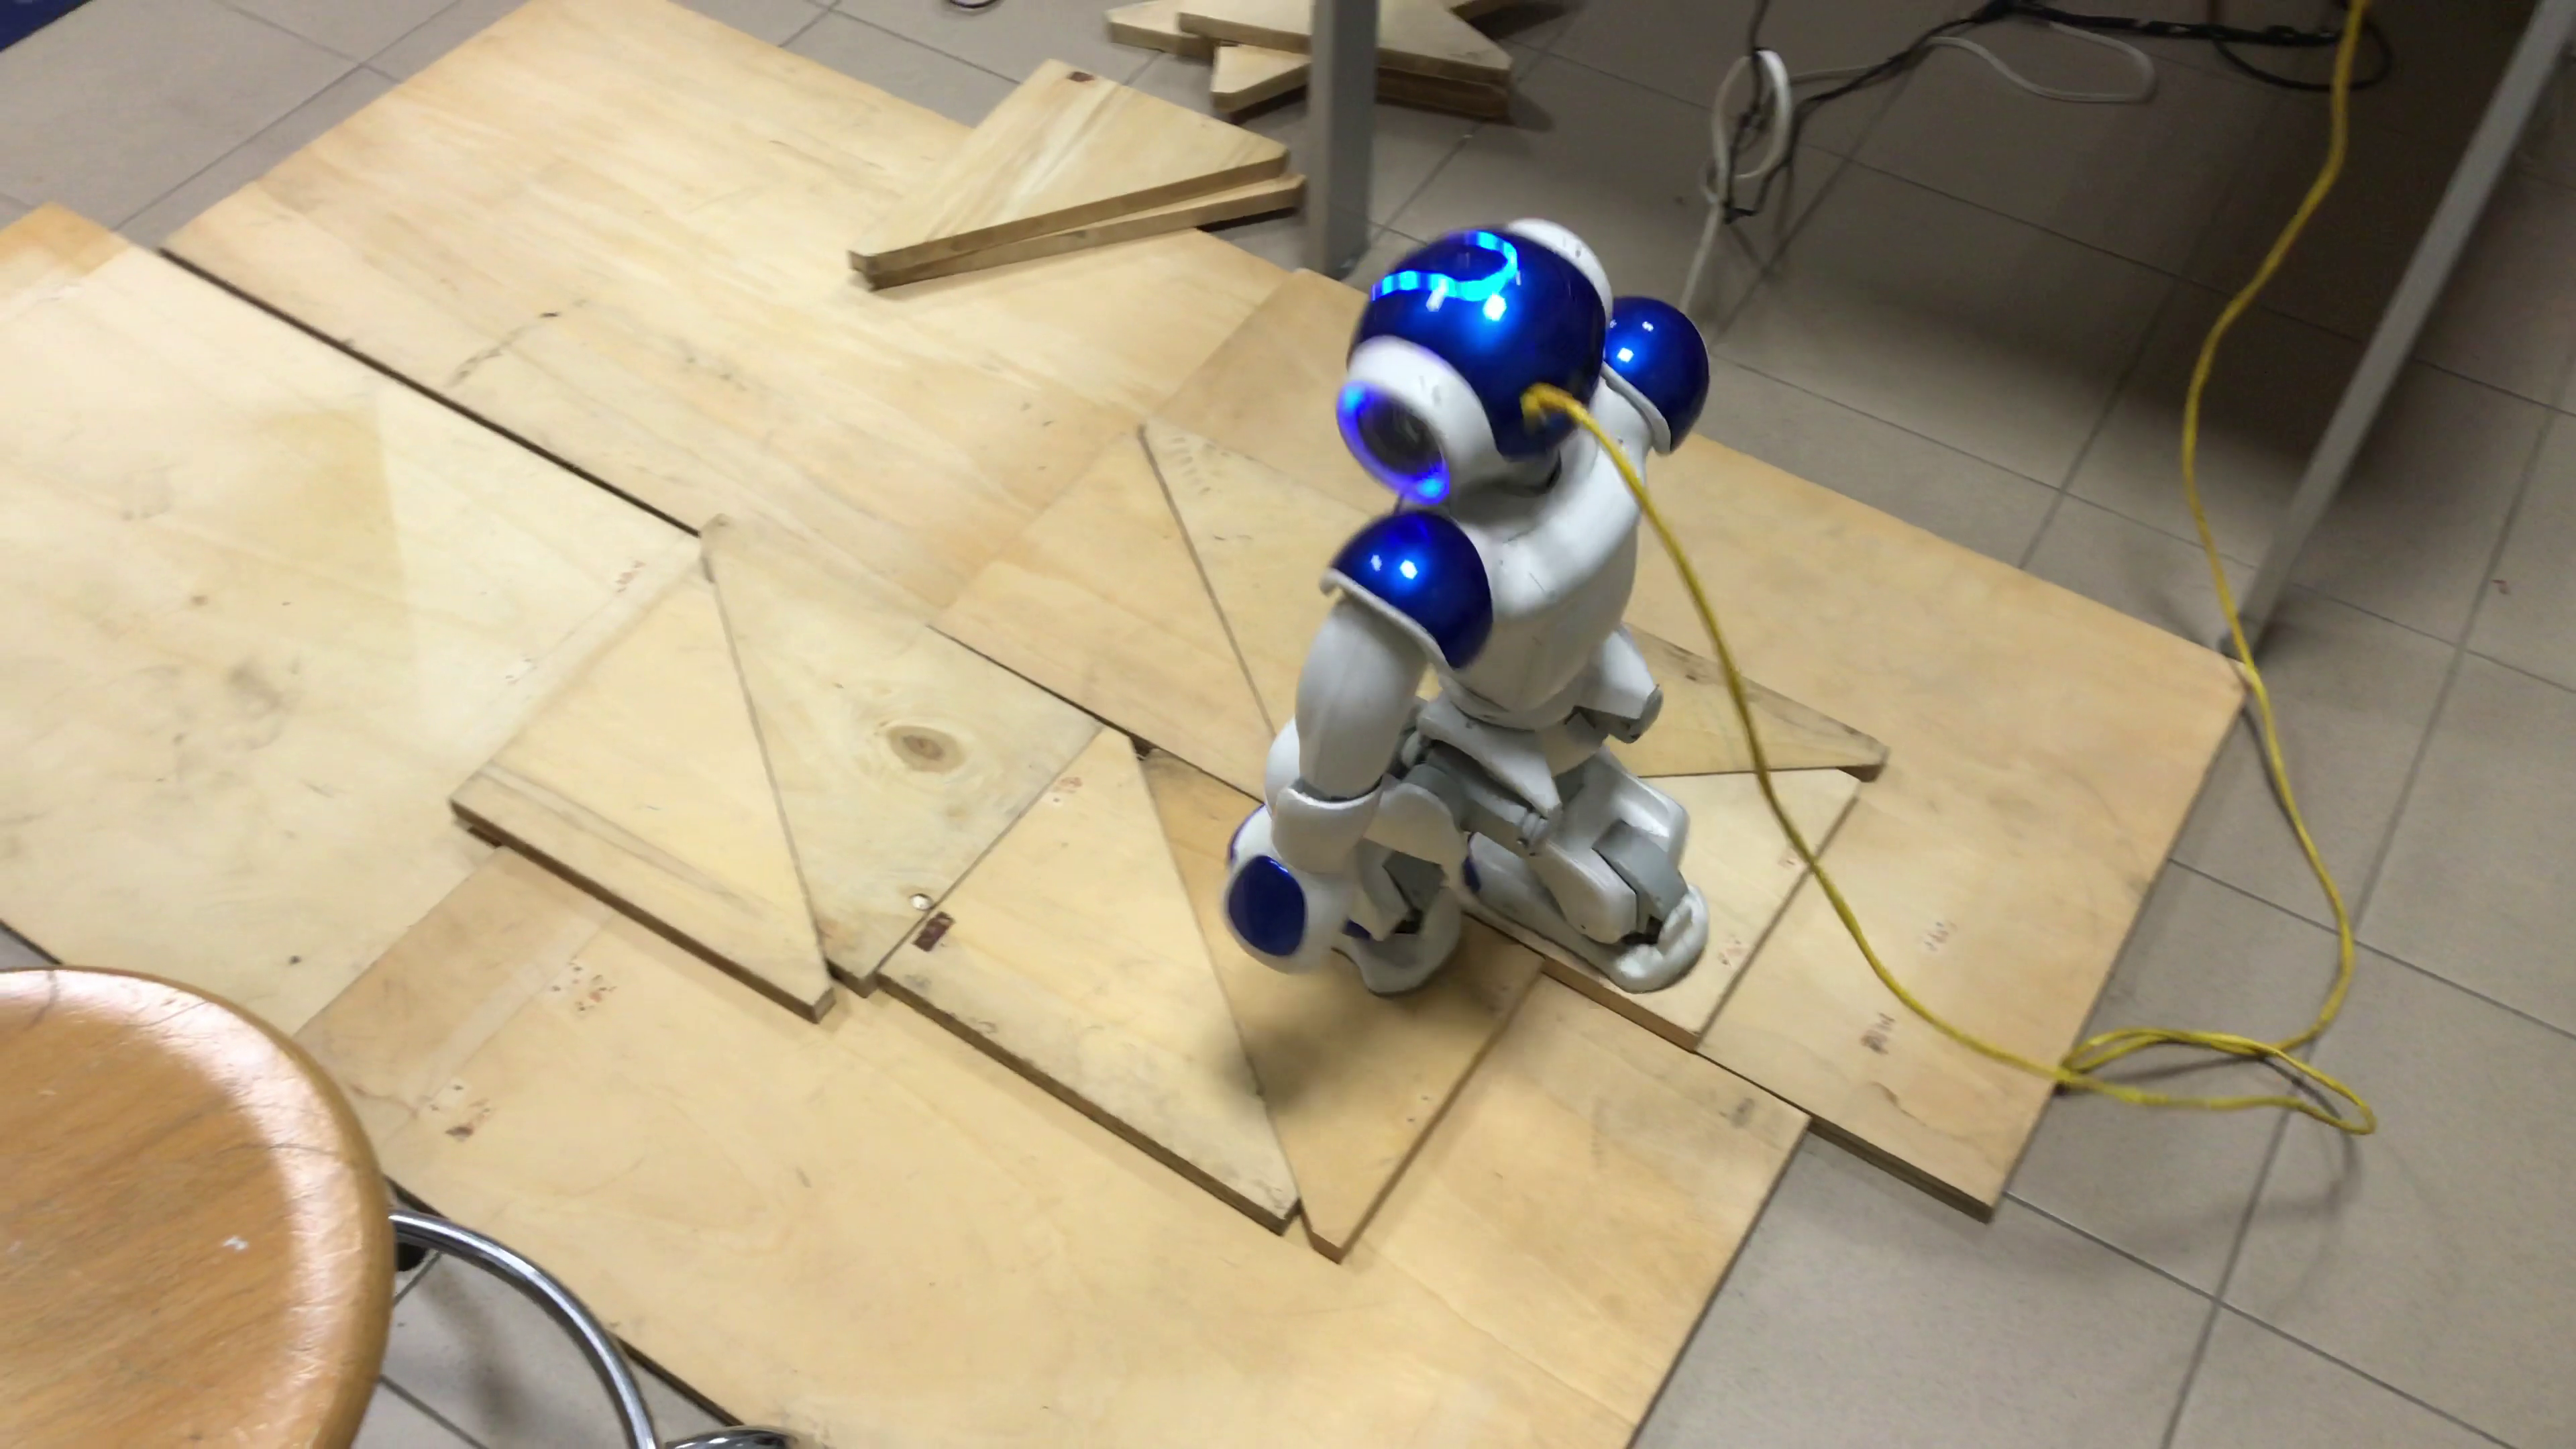
\includegraphics[width=\linewidth]
      {figures/experiments/multiple-staircases/upstairs/video/06.png}
    \caption{Fifth step}
  \end{subfigure}
  \caption{The figures show the motion of the robot for the scenario
      ``Multiple Staircases (Upstairs)''. The robot starts just in 
      front of the stairs (Fig. \ref{fig:exp:ms:up:frame1}), then it places 
      each step one in front of the other without colliding with the staircases,
      safely climbing the stairway. Each staircase has a height of 2 cm.}
  \label{fig:experiments:multiple-staircases:upstairs:videoframes}
\end{figure}

\begin{figure}
  \centering
  \includegraphics[width=\textwidth]
      {figures/experiments/multiple-staircases/upstairs/xy-plot-2cm.pdf}
  \includegraphics[width=\textwidth]
      {figures/experiments/multiple-staircases/upstairs/xz-plot-2cm.pdf}
  \caption{The plots show how the CoM and the ZMP vary with respect to the
		footsteps in the scenario ``Multiple Staircases (Upstairs)''.
    The green boxes represent the footsteps.}
  \label{fig:experiments:multiple-staircases:upstairs:comzmp}
\end{figure}

\subsection{Downstairs}
Downstairs.
\begin{figure}
  \begin{subfigure}{0.48\textwidth}
    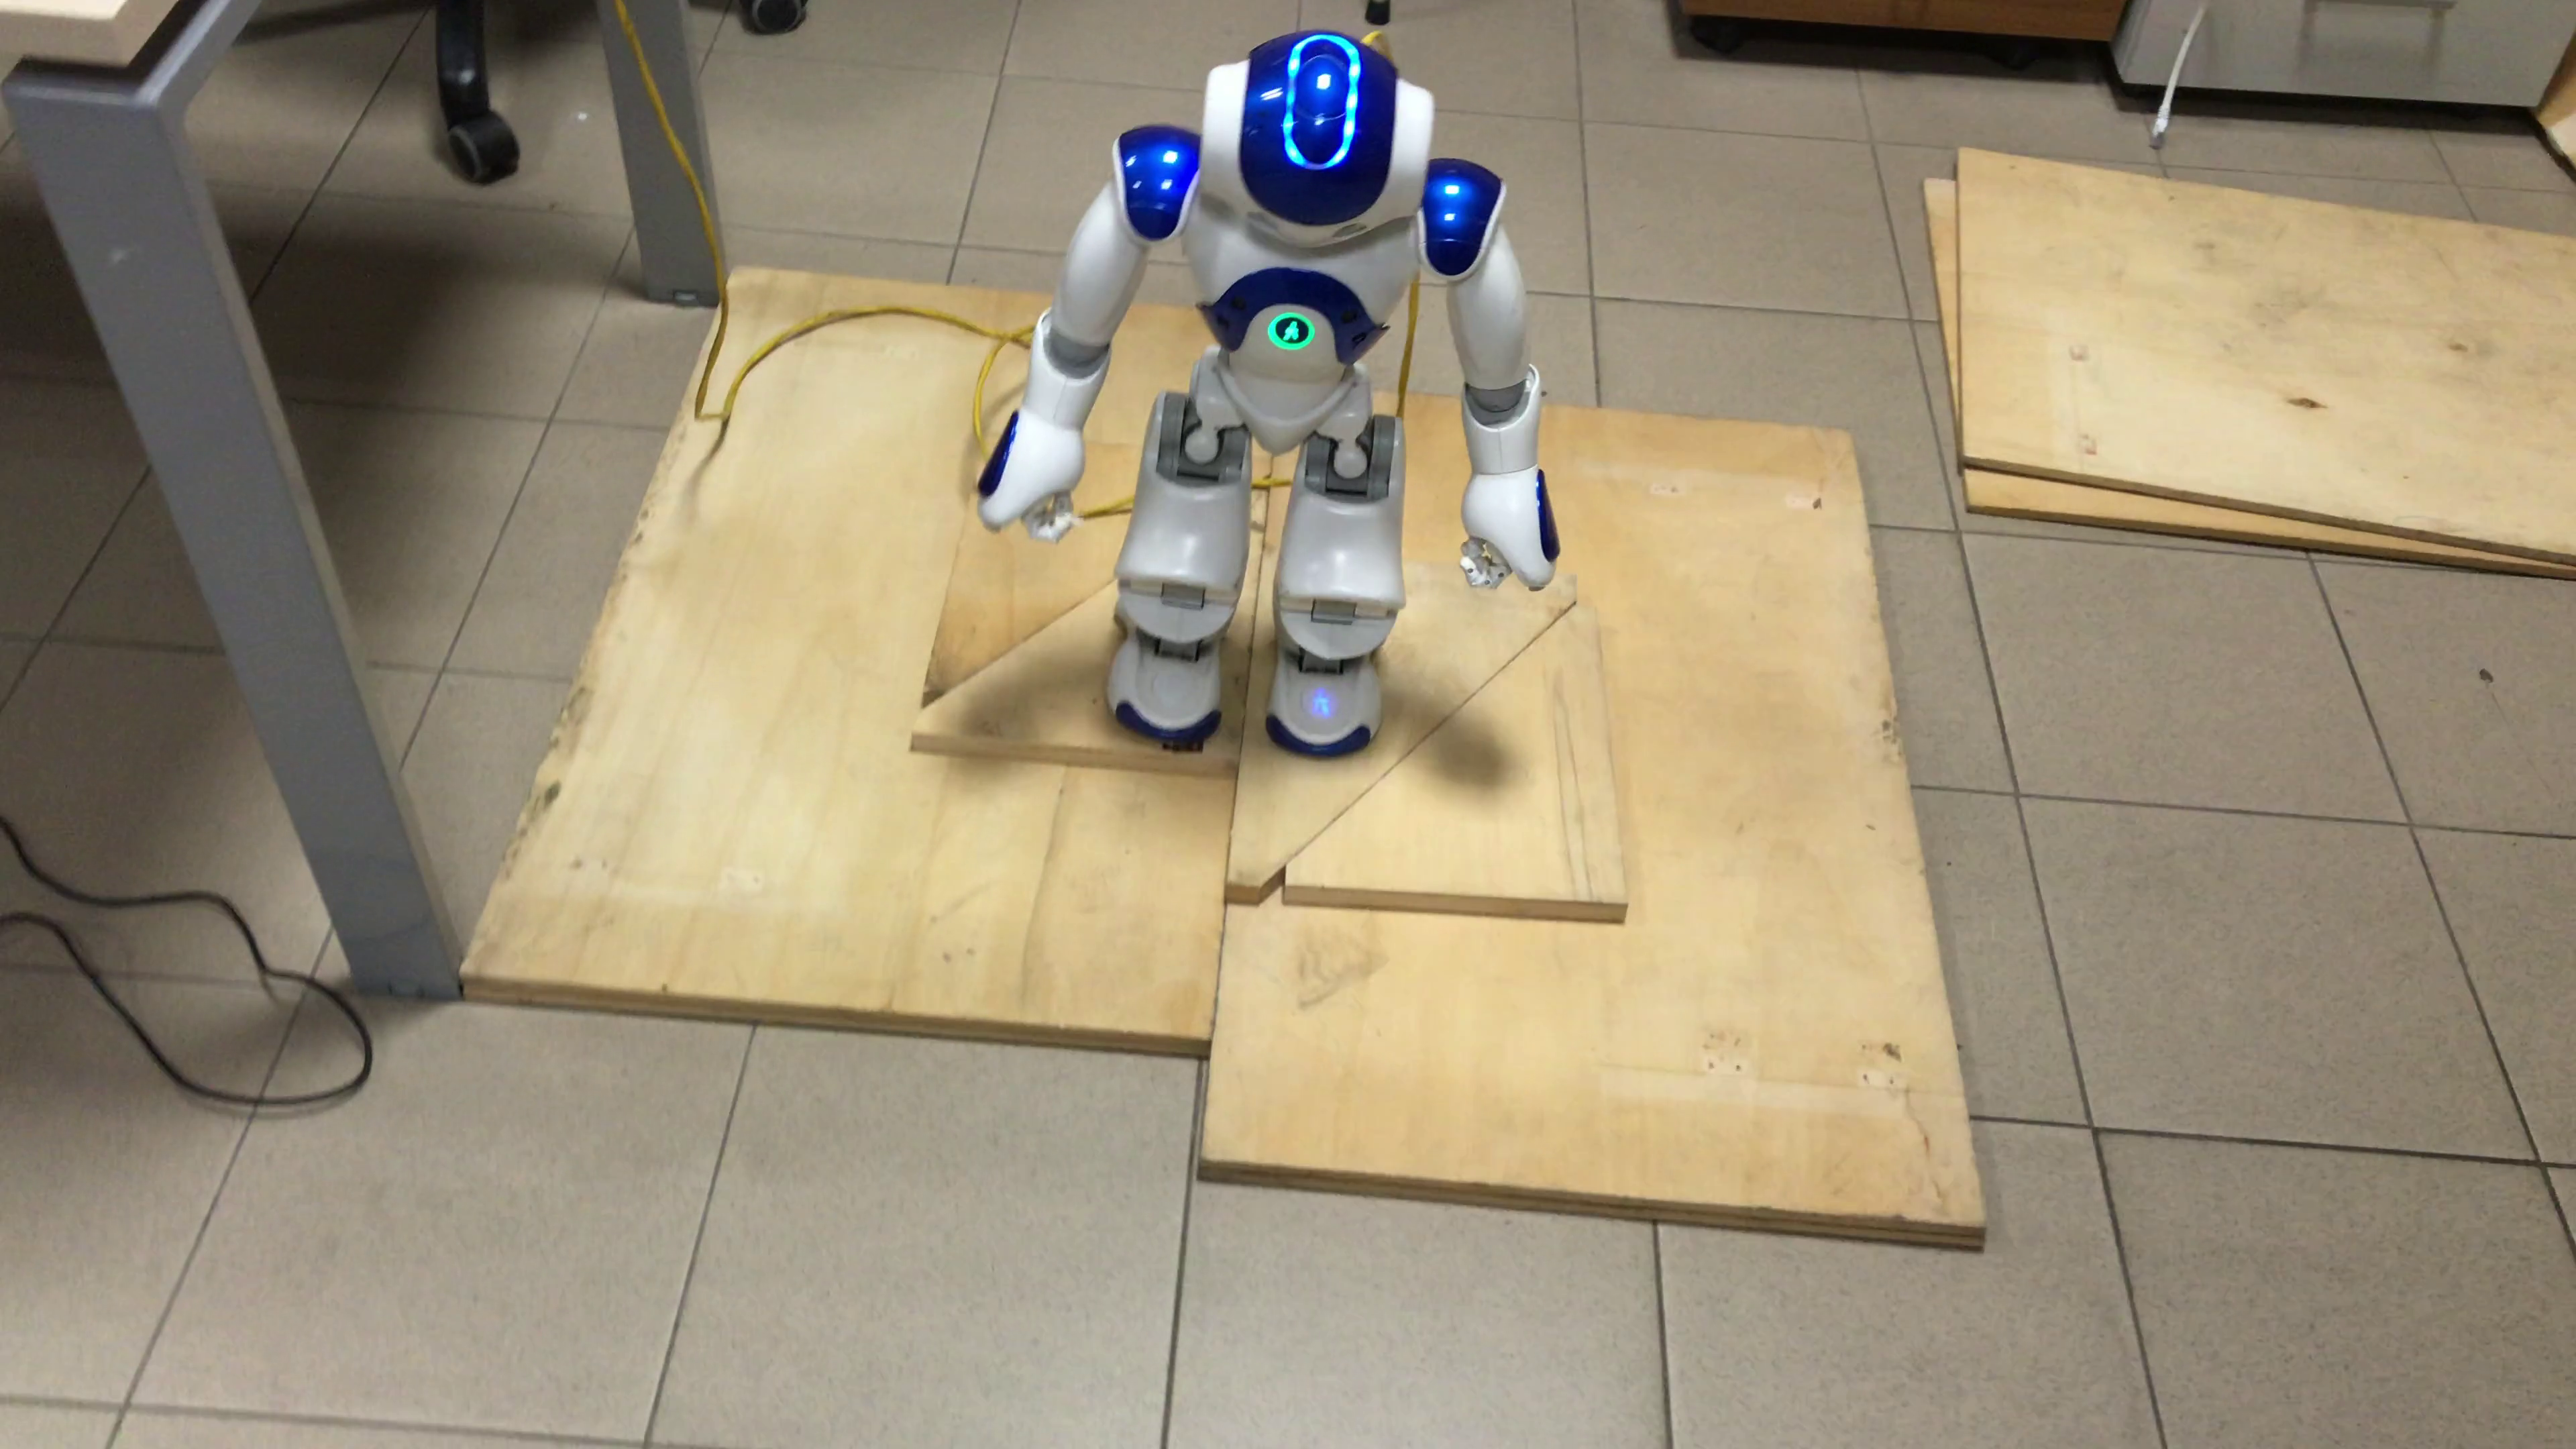
\includegraphics[width=\linewidth]
      {figures/experiments/multiple-staircases/downstairs/video/01.png}
    \caption{Starting position}
    \label{fig:exp:ms:down:frame1}
  \end{subfigure}\hspace*{\fill}
  \begin{subfigure}{0.48\textwidth}
    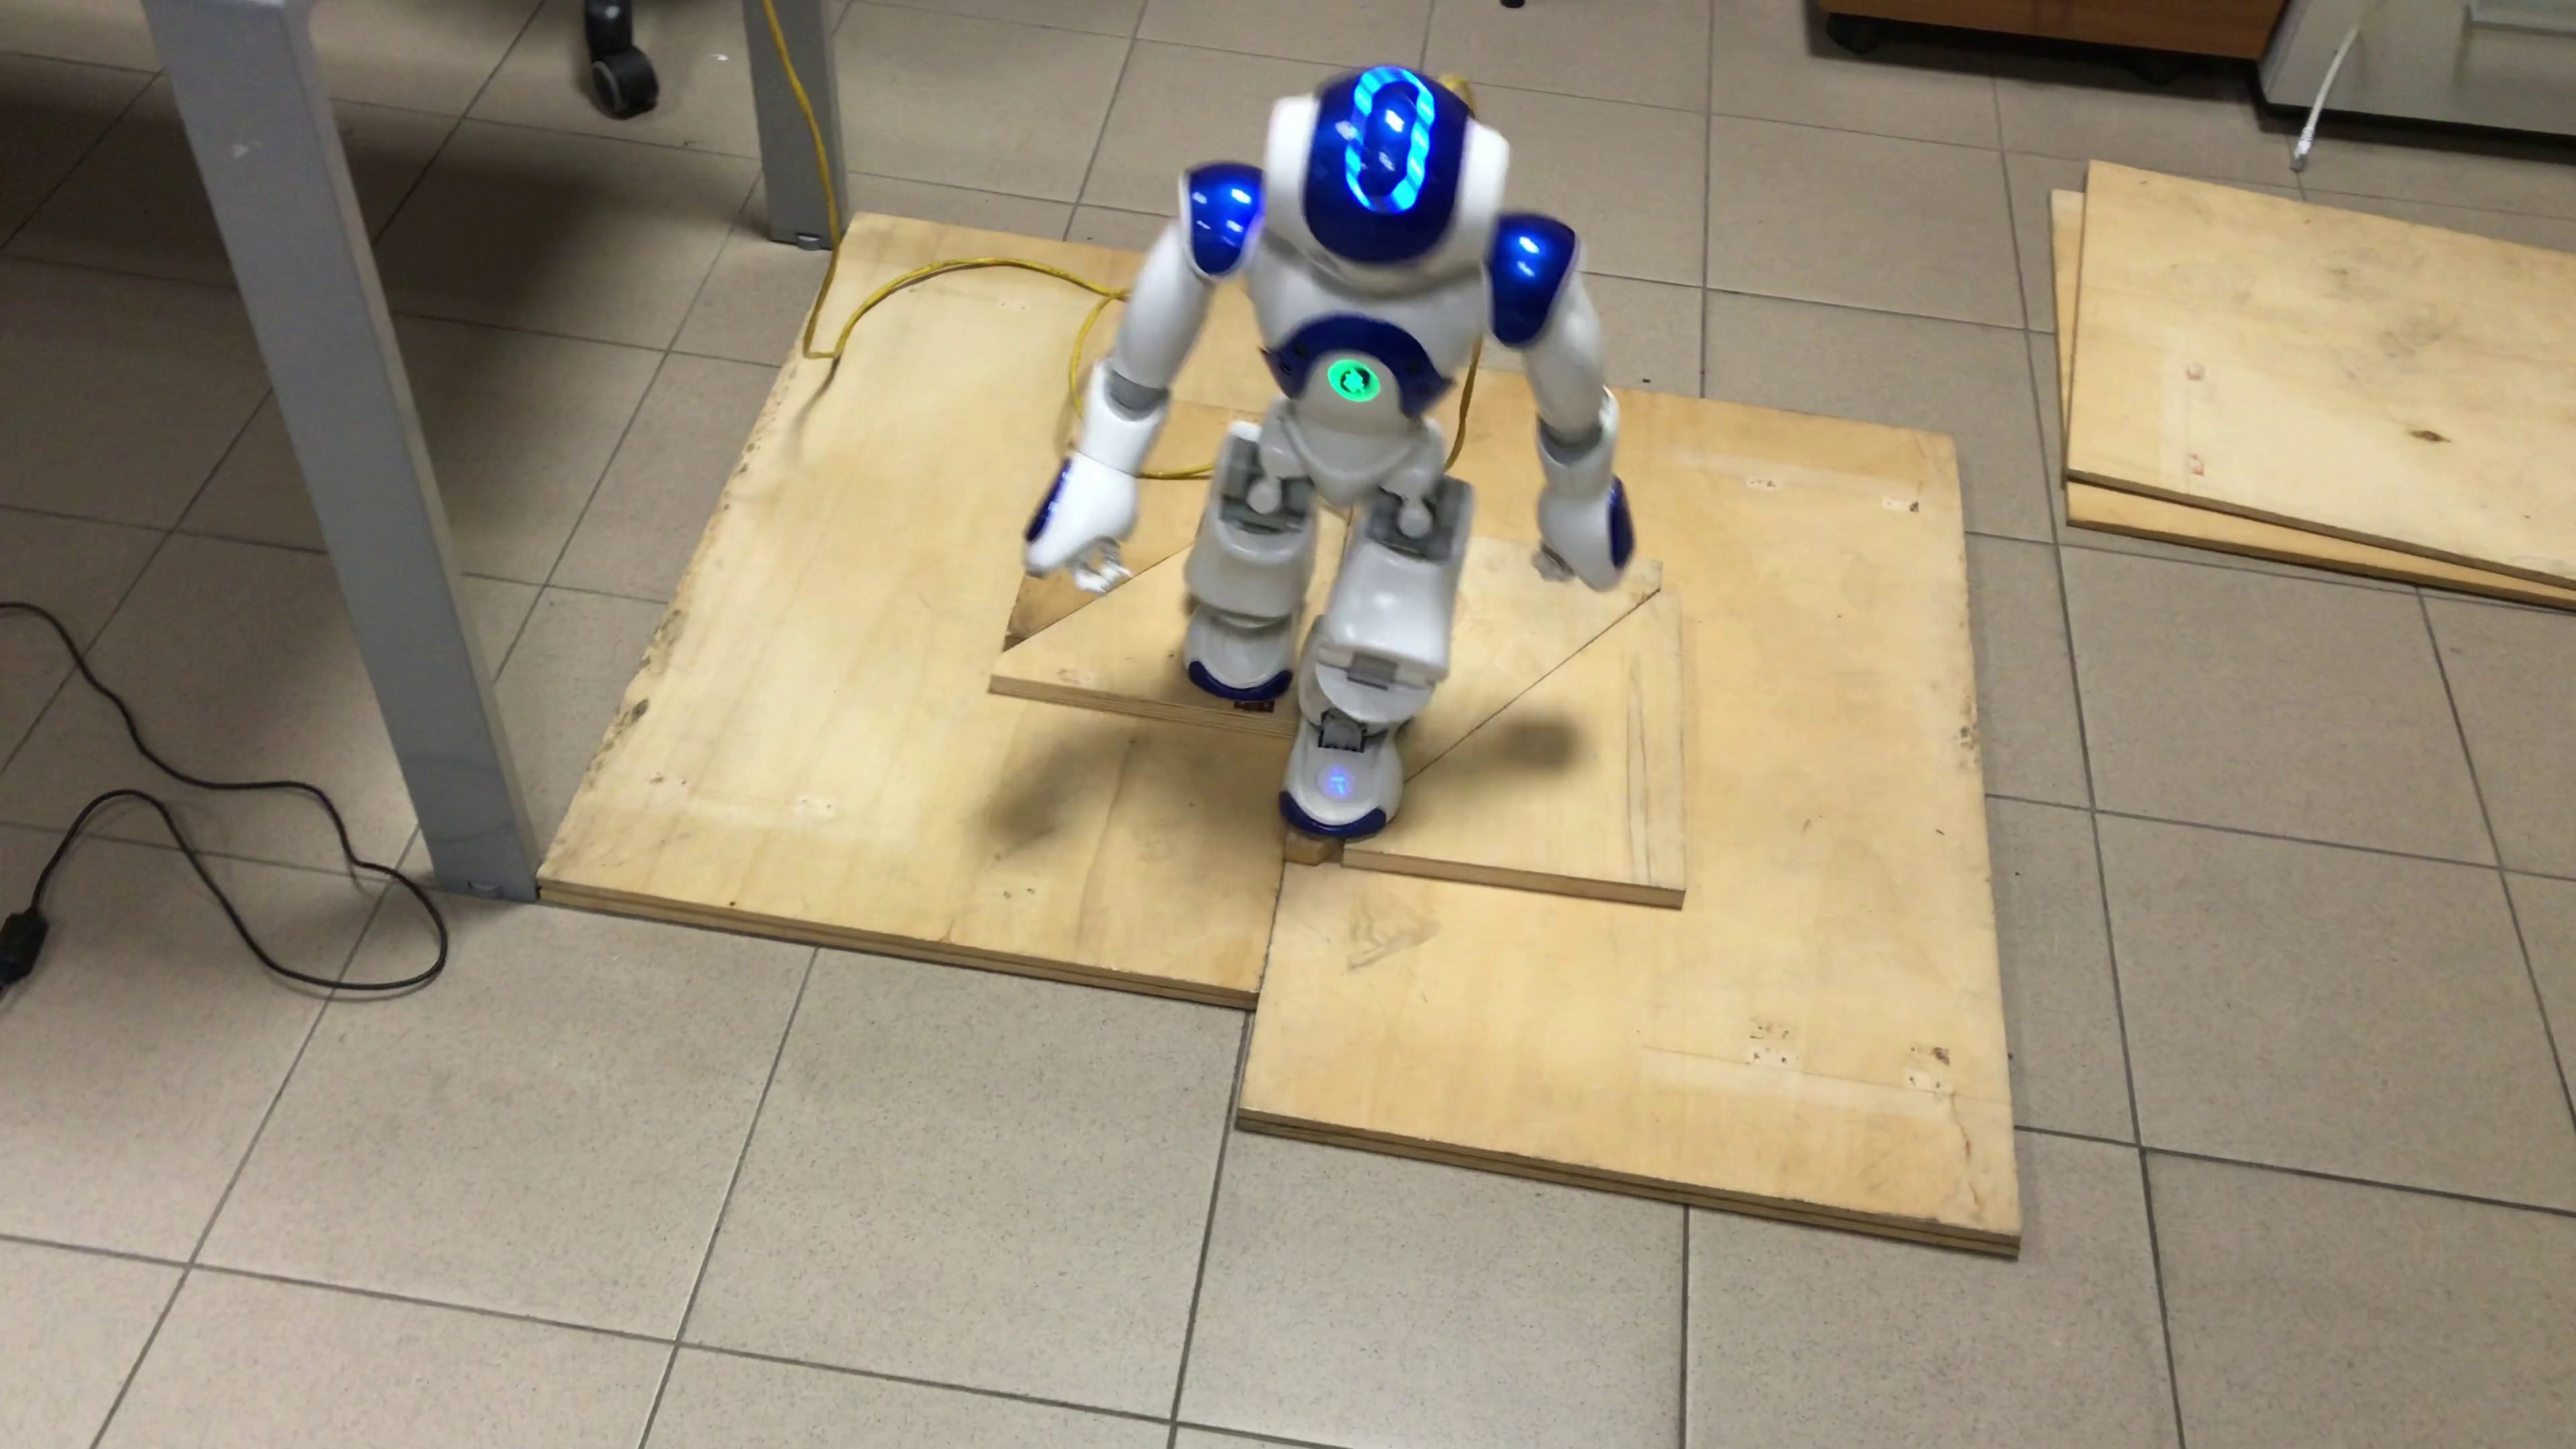
\includegraphics[width=\linewidth]
      {figures/experiments/multiple-staircases/downstairs/video/02.png}
    \caption{First step}
  \end{subfigure}
  \begin{subfigure}{0.48\textwidth}
    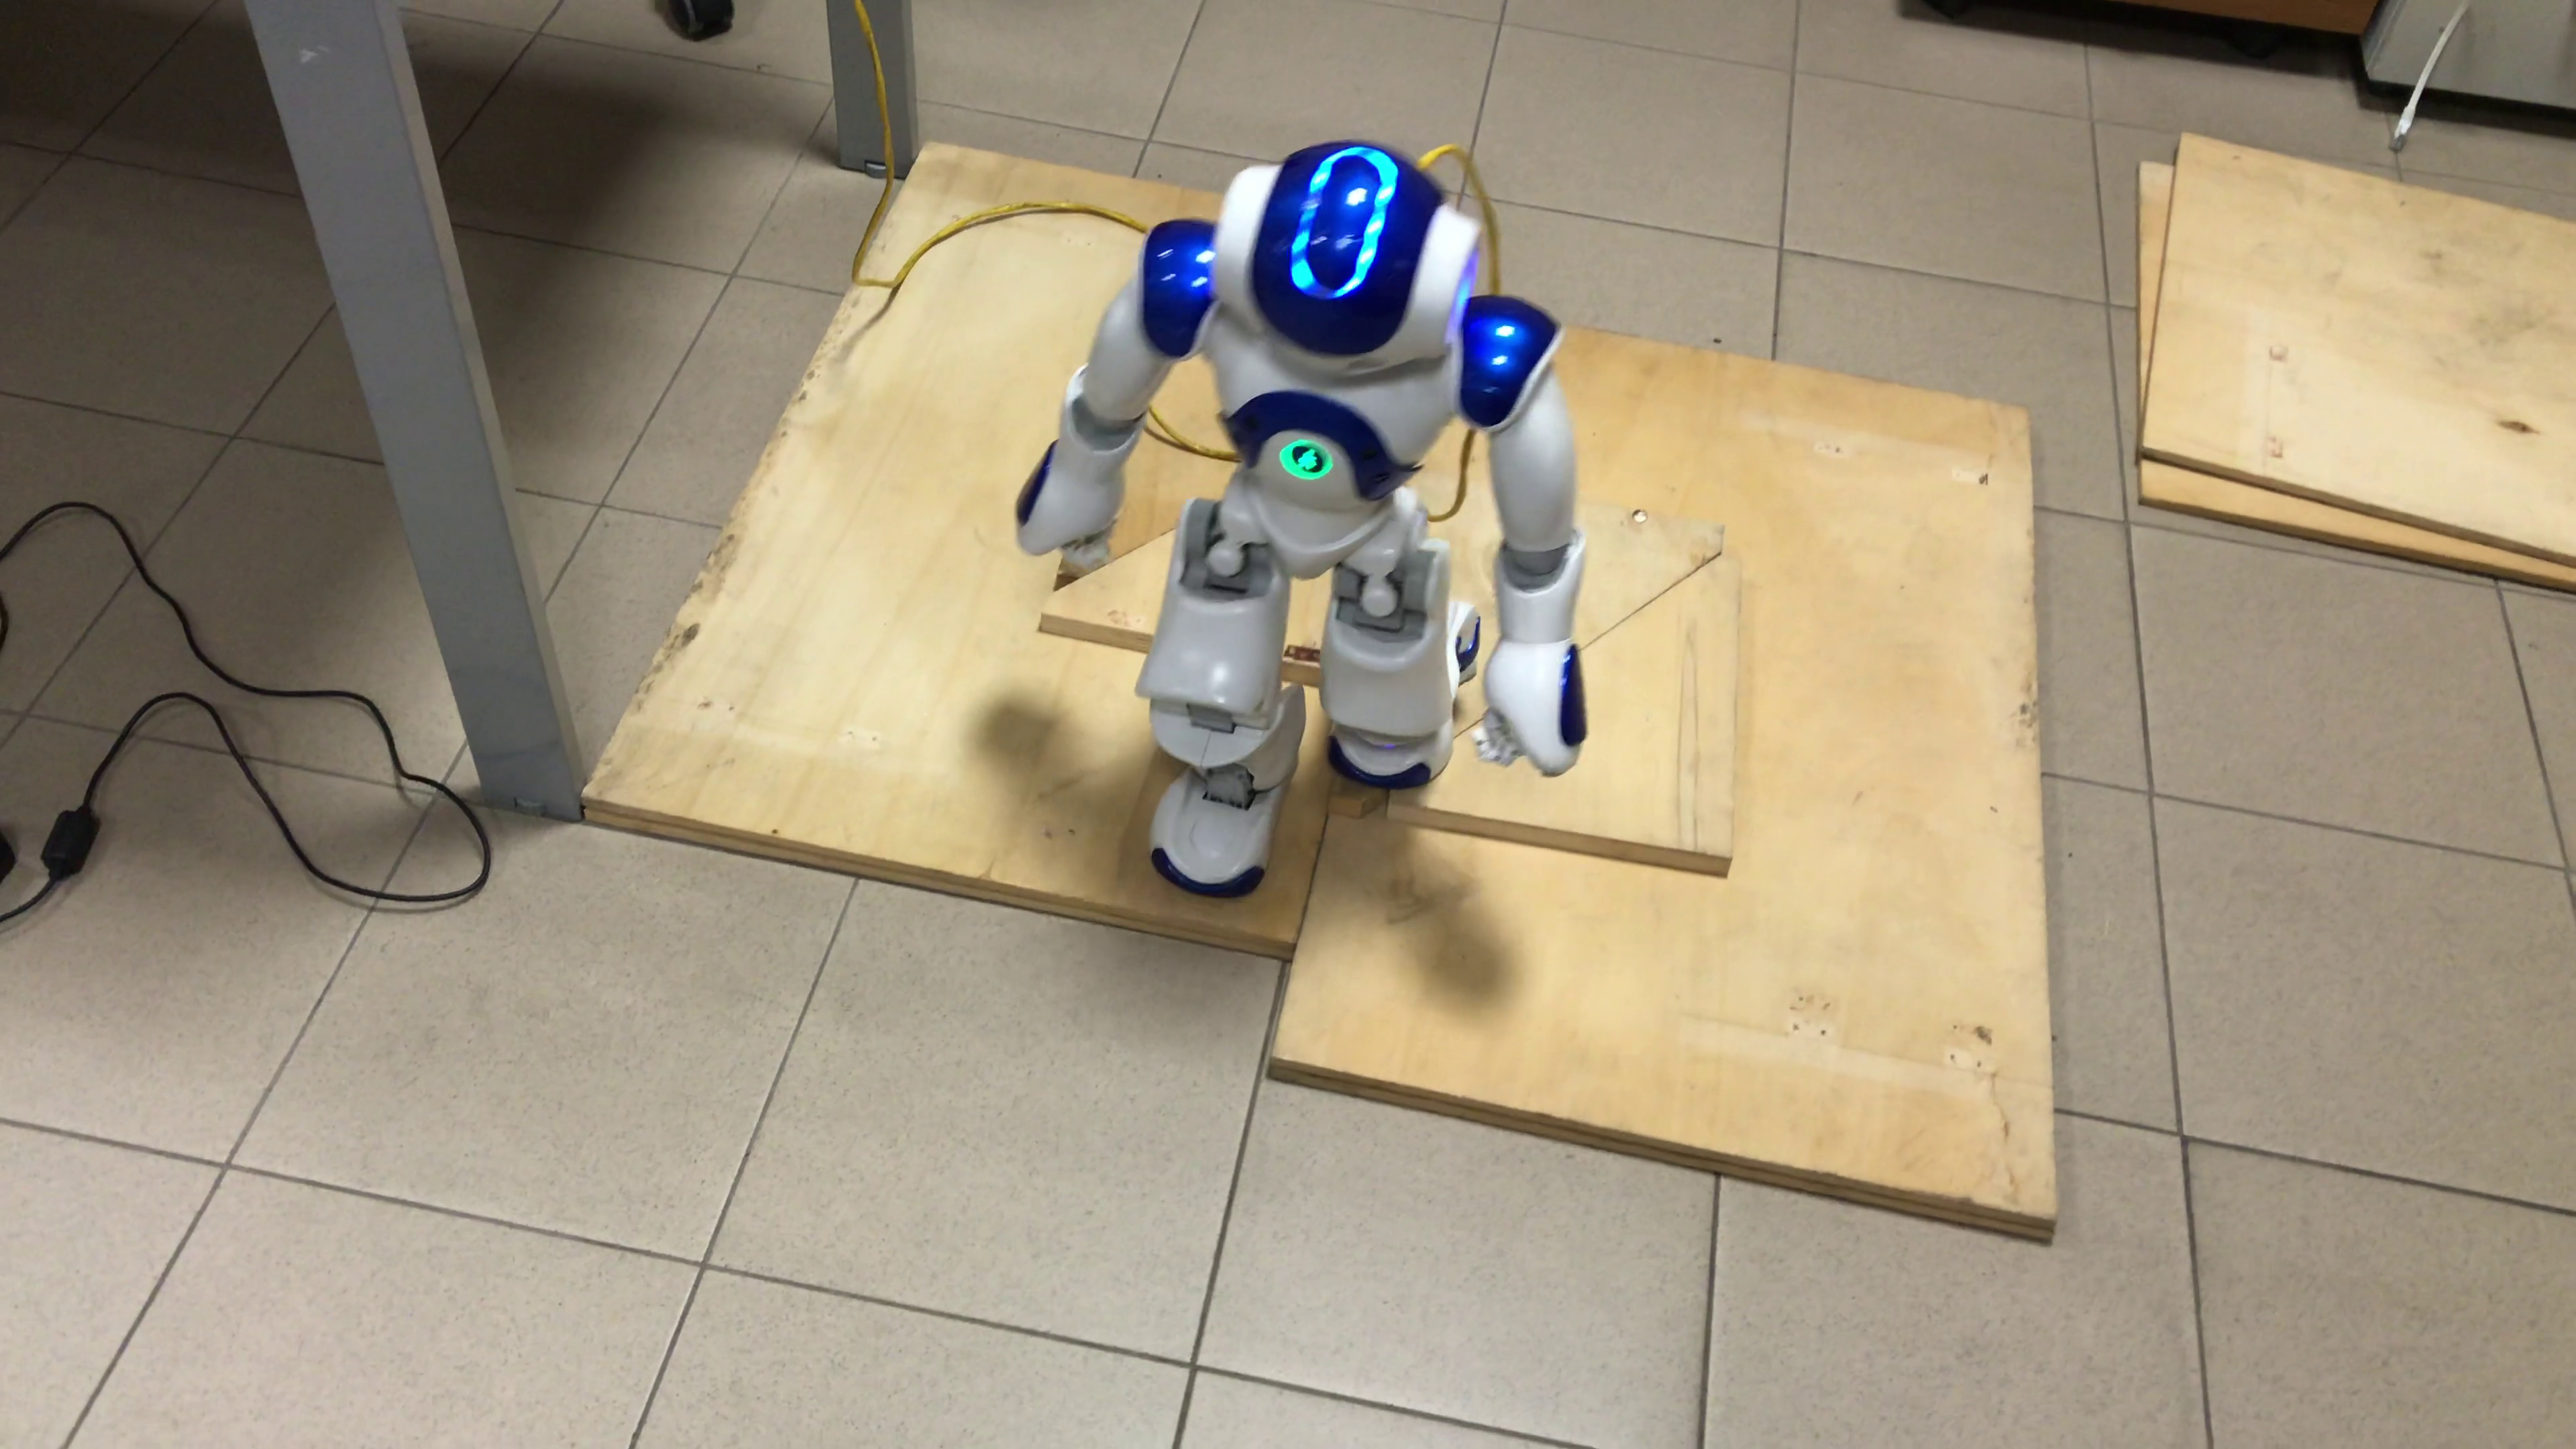
\includegraphics[width=\linewidth]
      {figures/experiments/multiple-staircases/downstairs/video/03.png}
    \caption{Second step}
  \end{subfigure}\hspace*{\fill}
  \begin{subfigure}{0.48\textwidth}
    \includegraphics[width=\linewidth]
      {figures/experiments/multiple-staircases/downstairs/video/04.png}
    \caption{Third step}
  \end{subfigure}
  \begin{subfigure}{0.48\textwidth}
    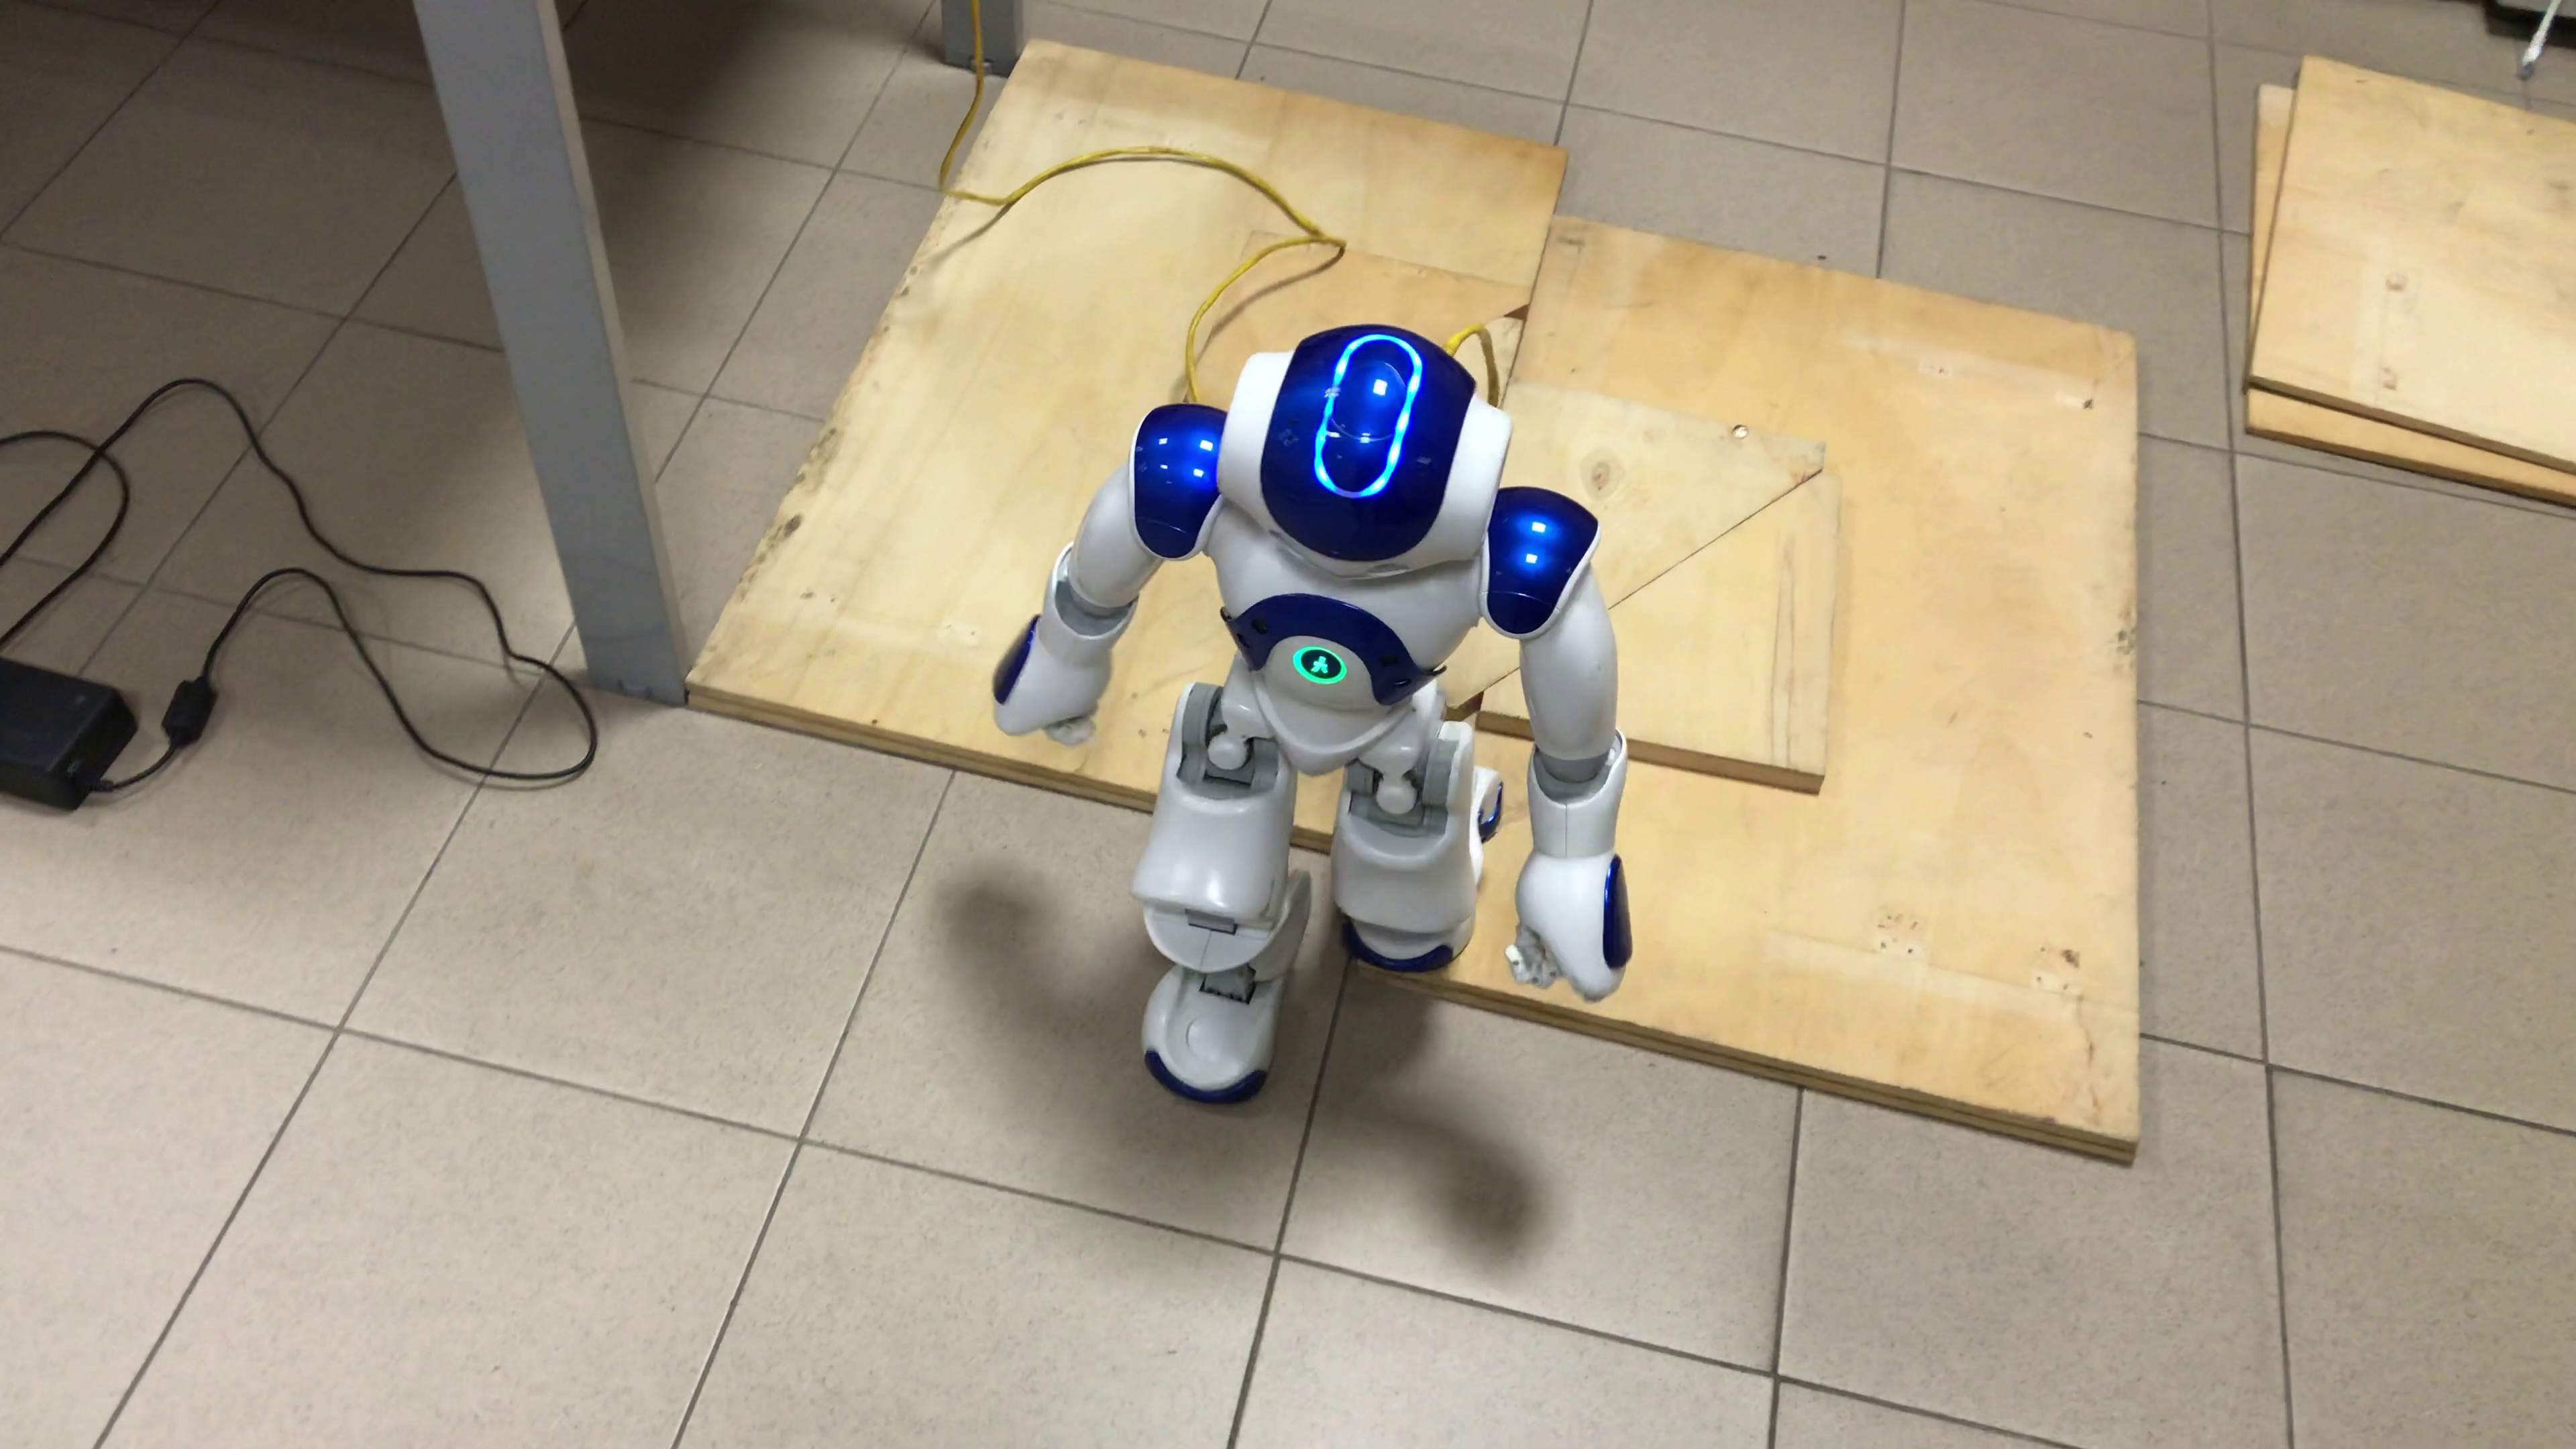
\includegraphics[width=\linewidth]
      {figures/experiments/multiple-staircases/downstairs/video/05.png}
    \caption{Fourth step}
  \end{subfigure}\hspace*{\fill}
  \begin{subfigure}{0.48\textwidth}
    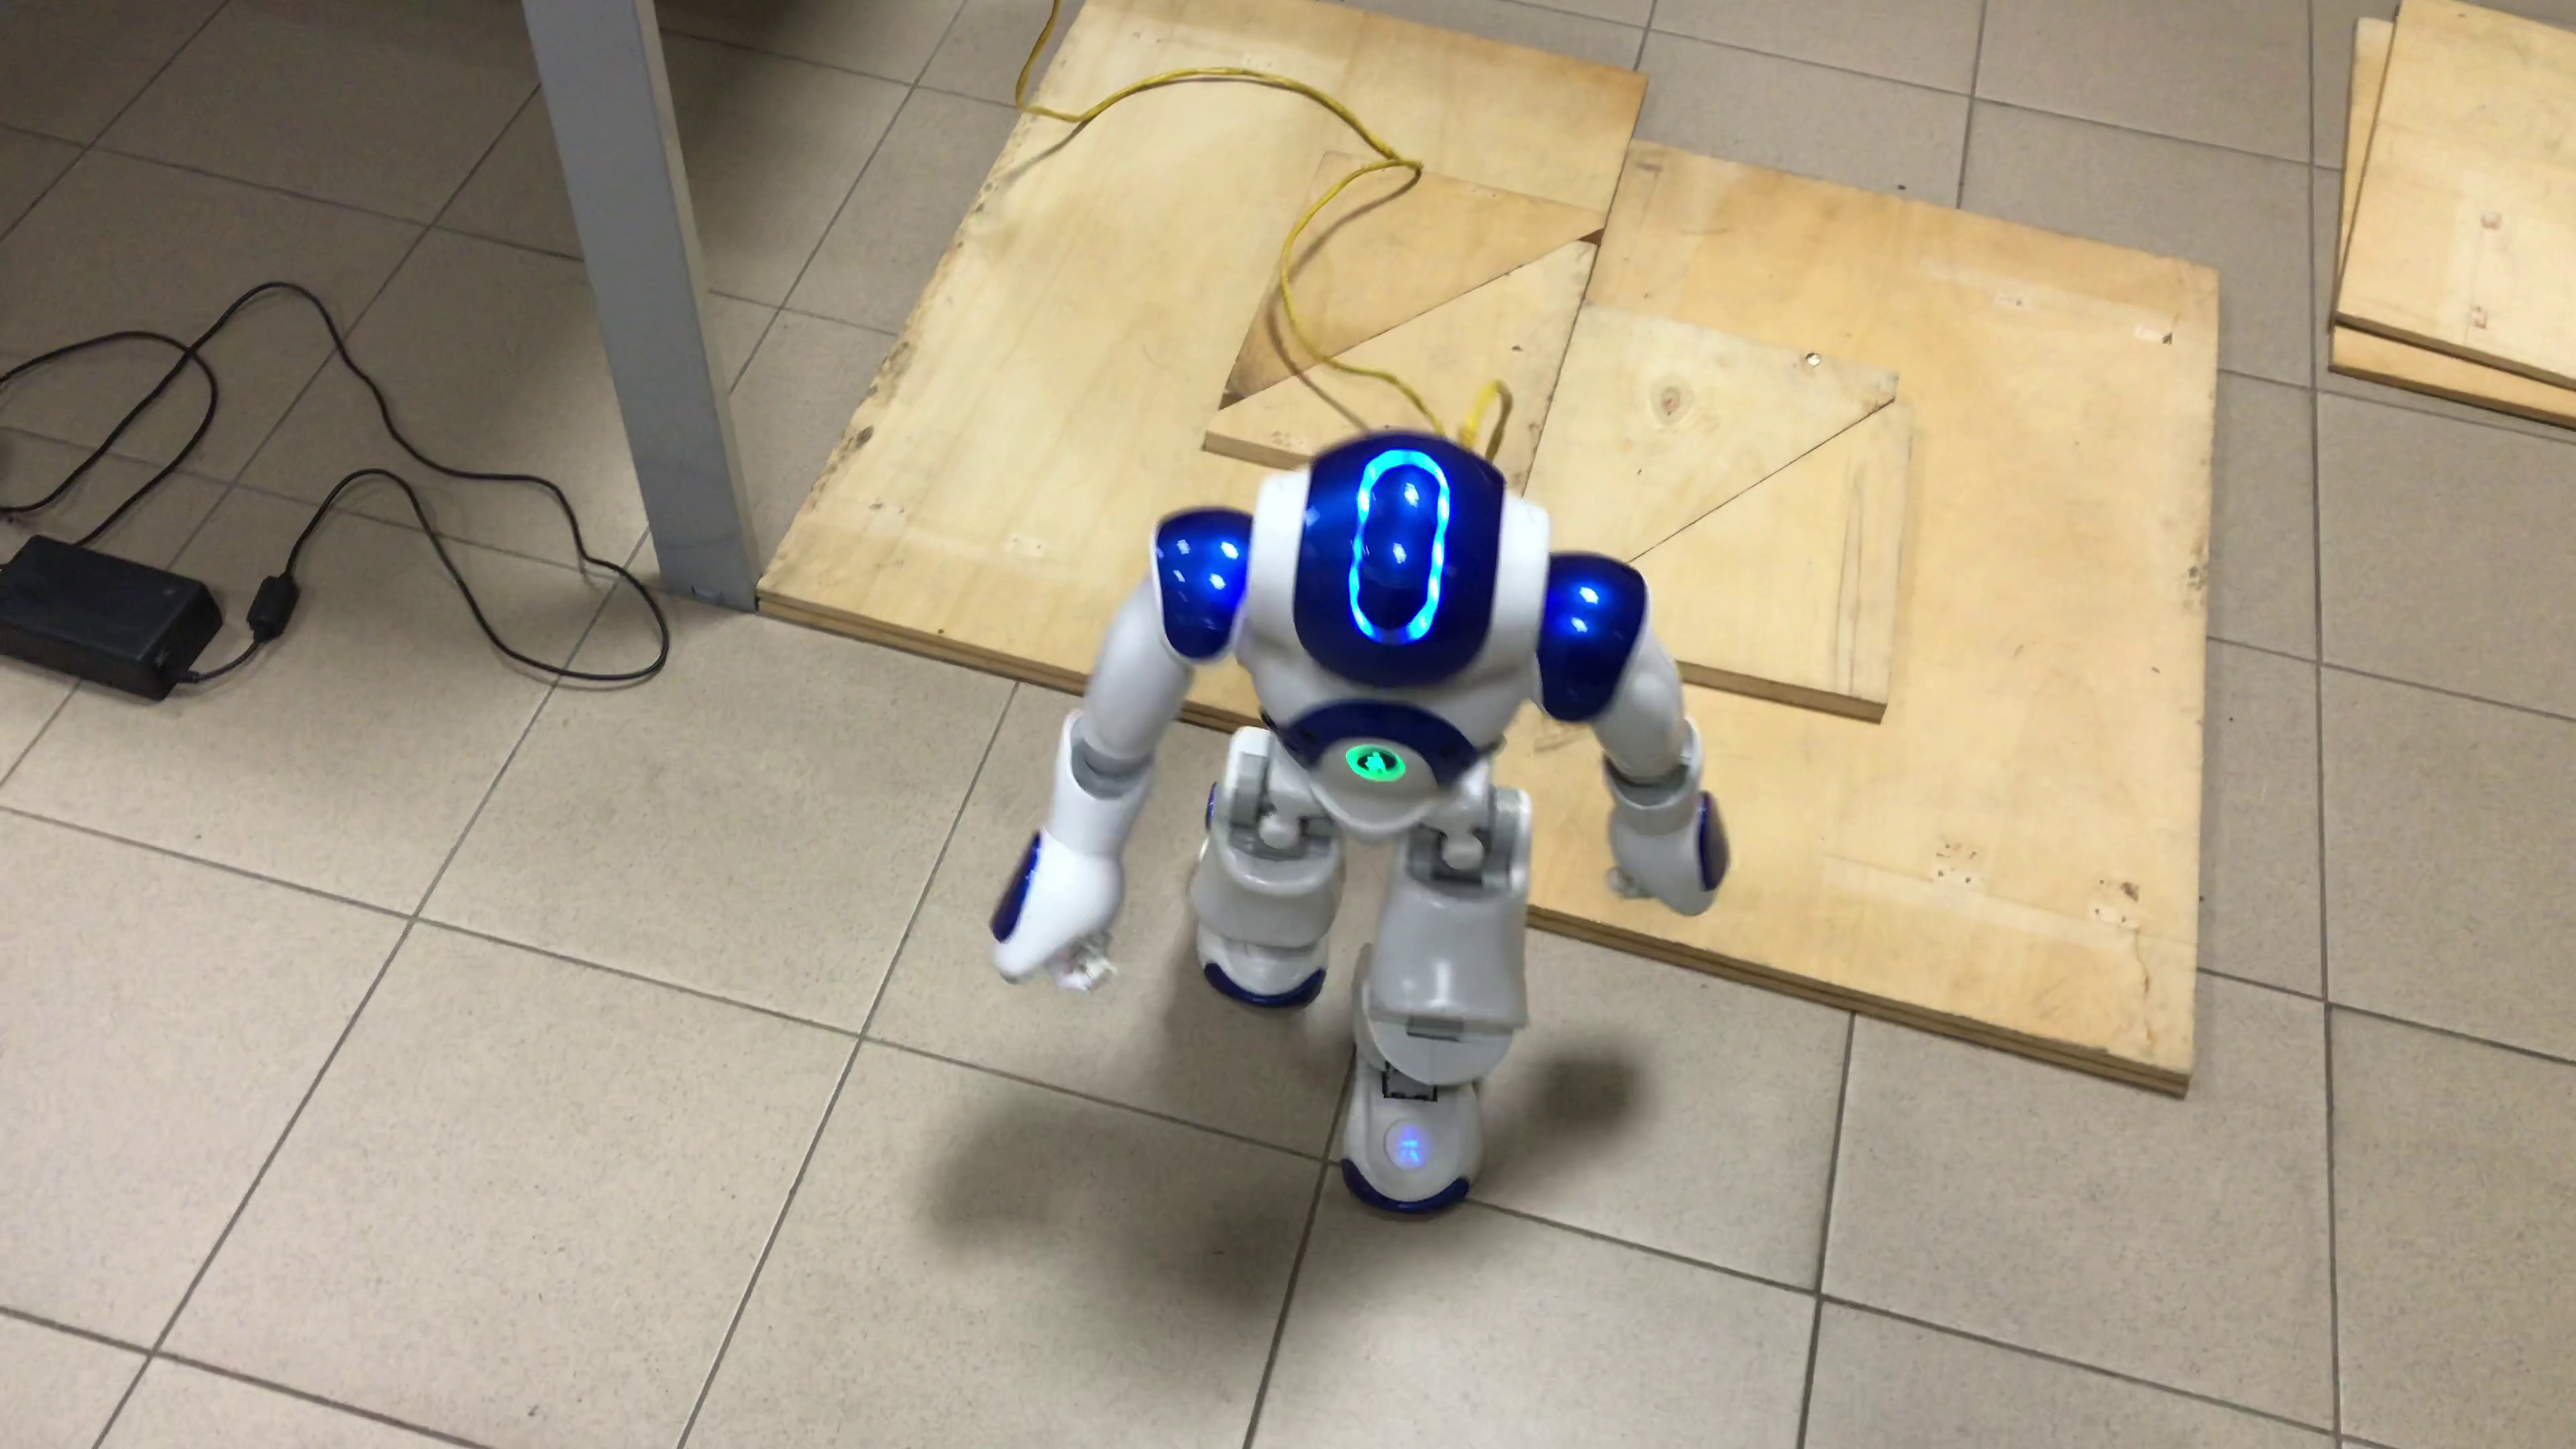
\includegraphics[width=\linewidth]
      {figures/experiments/multiple-staircases/downstairs/video/06.png}
    \caption{Fifth step}
  \end{subfigure}
  \caption{The figures show the motion of the robot for the scenario
      ``Multiple Staircases (Downstairs)''. The robot starts on top of the 
      stairway (Fig. \ref{fig:exp:ms:down:frame1}), then it places 
      each step one in front of the other without colliding with the staircases,
      safely reaching ground level. Each staircase has a height of 2 cm.}
  \label{fig:experiments:multiple-staircases:downstairs:videoframes}
\end{figure}

\begin{figure}
  \centering
  \includegraphics[width=\textwidth]
      {figures/experiments/multiple-staircases/downstairs/xy-plot-2cm.pdf}
  \includegraphics[width=\textwidth]
      {figures/experiments/multiple-staircases/downstairs/xz-plot-2cm.pdf}
  \caption{The plots show how the CoM and the ZMP vary with respect to the
		footsteps in the scenario ``Multiple Staircases (Downstairs)''.
    The green boxes represent the footsteps.}
  \label{fig:experiments:multiple-staircases:downstairs:comzmp}
\end{figure}

\section{Obstacle Avoidance}
Footstep planning with manually generated elevation mapping. Map contains 
an obstacle that can not be climbed by NAO because of short legs.
\begin{figure}
  \begin{subfigure}{0.48\textwidth}
    \includegraphics[width=\linewidth]
      {figures/experiments/obstacle-avoidance/video/01.png}
    \caption{Starting position}
    \label{fig:exp:obs:frame1}
  \end{subfigure}\hspace*{\fill}
  \begin{subfigure}{0.48\textwidth}
    \includegraphics[width=\linewidth]
      {figures/experiments/obstacle-avoidance/video/02.png}
    \caption{Moving to the left}
    \label{fig:exp:obs:frame2}
  \end{subfigure}
  \begin{subfigure}{0.48\textwidth}
    \includegraphics[width=\linewidth]
      {figures/experiments/obstacle-avoidance/video/03.png}
    \caption{Avoiding the obstacle}
  \end{subfigure}\hspace*{\fill}
  \begin{subfigure}{0.48\textwidth}
    \includegraphics[width=\linewidth]
      {figures/experiments/obstacle-avoidance/video/04.png}
    \caption{Moving forward}
  \end{subfigure}
  \begin{subfigure}{0.48\textwidth}
    \includegraphics[width=\linewidth]
      {figures/experiments/obstacle-avoidance/video/05.png}
    \caption{Moving towards the goal}
    \label{fig:exp:obs:frame5}
  \end{subfigure}\hspace*{\fill}
  \begin{subfigure}{0.48\textwidth}
    \includegraphics[width=\linewidth]
      {figures/experiments/obstacle-avoidance/video/06.png}
    \caption{Goal region reached}
    \label{fig:exp:obs:frame6}
  \end{subfigure}
  \caption{The figures show the motion of the robot for the scenario
      ``Obstacle Avoidance''. The robot starts in front of the obstacle
      (Fig. \ref{fig:exp:obs:frame1}), then it moves to its left correctly
      avoiding it (Fig. \ref{fig:exp:obs:frame2}-\ref{fig:exp:obs:frame5})
      until it reaches the goal region (Fig. \ref{fig:exp:obs:frame6}),
      whose center is represented by 
      the ball. The goal region is a circle with a radius of 10 cm. 
      Note that even if the obstacle has a height of 2 cm, NAO can not climb it 
      because of its kinematic limitations, hence, the planner takes
      into account the mechanical capabilities of the robot, generating a 
      safe and realizable footstep plan.}
  \label{fig:experiments:obstacle-avoidance:videoframes}
\end{figure}

\begin{figure}
    \centering
    \includegraphics[width=0.95\textwidth]
        {figures/experiments/obstacle-avoidance/footstep-plan.pdf}
    \caption{Footstep plan generated for the scenario ``Obstacle Avoidance''.}
    \label{fig:experiments:obstacle-avoidance:footstep-plan}
\end{figure}
\begin{figure}
    \centering
    \includegraphics[width=0.95\textwidth]
        {figures/experiments/obstacle-avoidance/rrt-tree.pdf}
    \caption{Tree generated for the scenario ``Obstacle Avoidance''.}
    \label{fig:experiments:obstacle-avoidance:rrt-tree}
\end{figure}

\section{Stair Climbing in Unknown Environment}
Stair climbing (unknown environment). Planner + \texttt{elevation\_mapping}.
\begin{figure}
  \begin{subfigure}{0.48\textwidth}
    \includegraphics[width=\linewidth]
      {figures/experiments/unknown-env/video/01.png}
    \caption{Starting position}
    \label{fig:exp:unkenv:frame1}
  \end{subfigure}\hspace*{\fill}
  \begin{subfigure}{0.48\textwidth}
    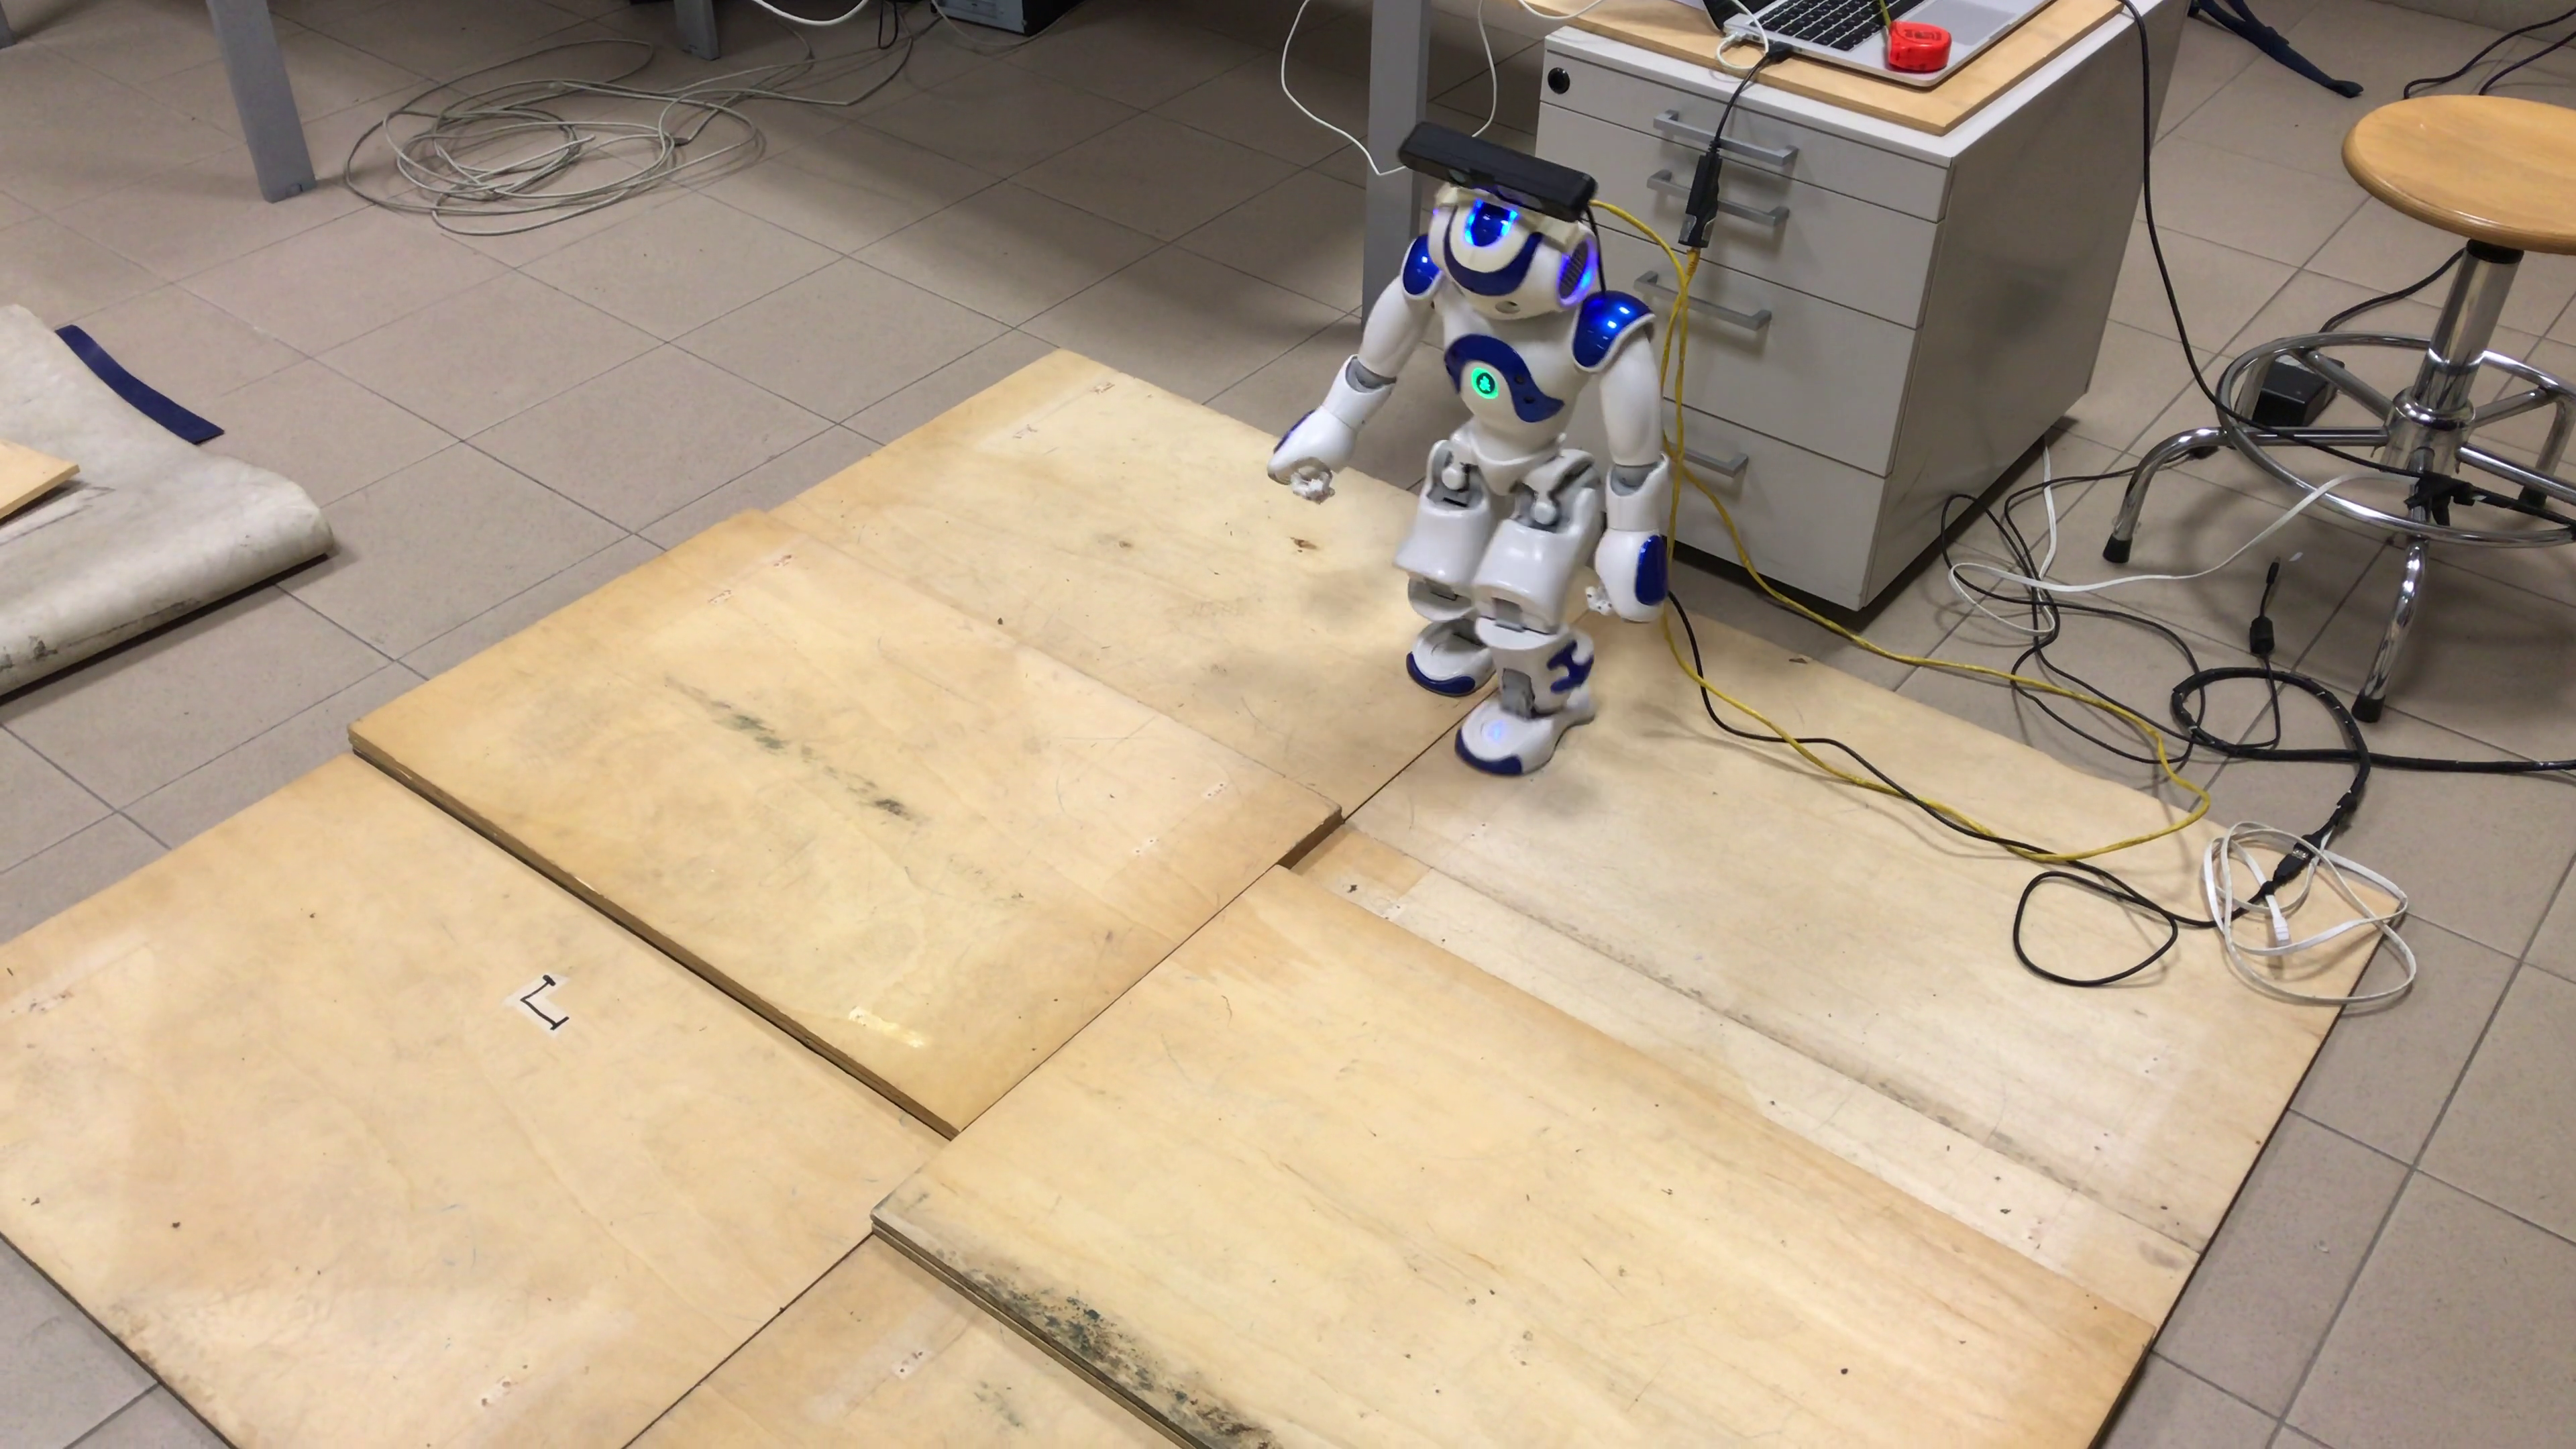
\includegraphics[width=\linewidth]
      {figures/experiments/unknown-env/video/02.png}
    \caption{First step}
    \label{fig:exp:unkenv:frame2}
  \end{subfigure}
  \begin{subfigure}{0.48\textwidth}
    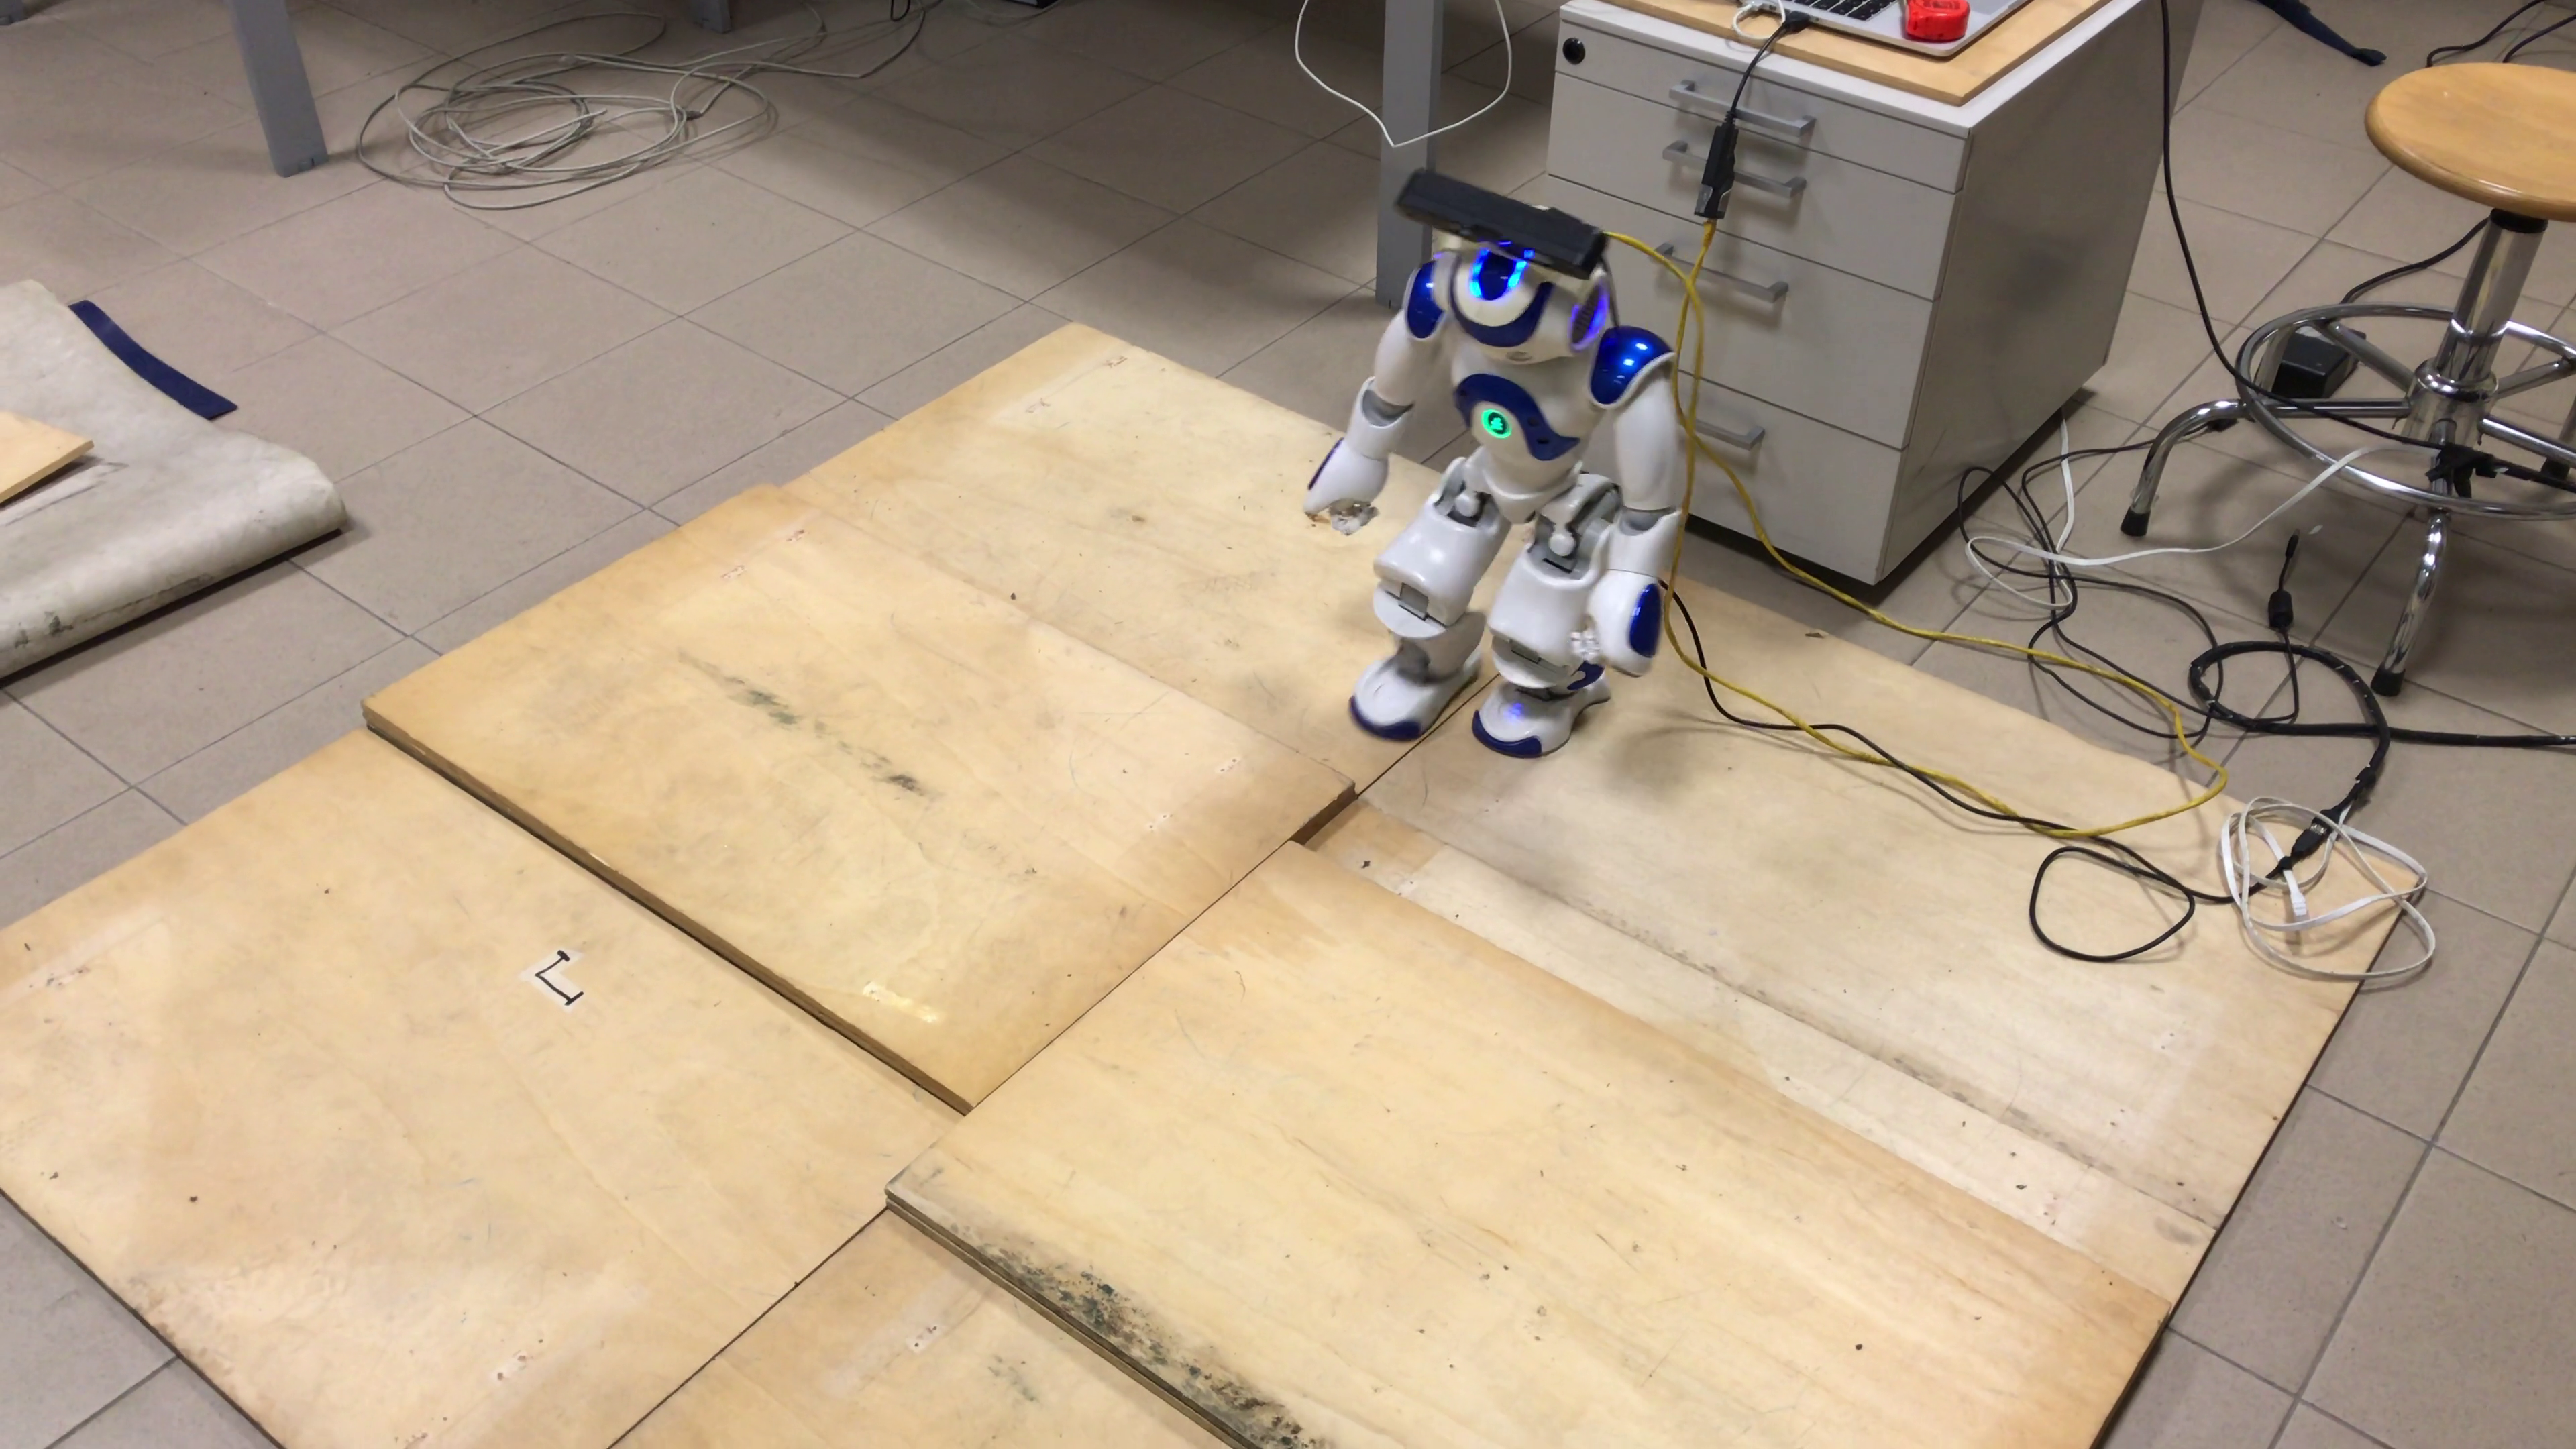
\includegraphics[width=\linewidth]
      {figures/experiments/unknown-env/video/03.png}
    \caption{Second step}
  \end{subfigure}\hspace*{\fill}
  \begin{subfigure}{0.48\textwidth}
    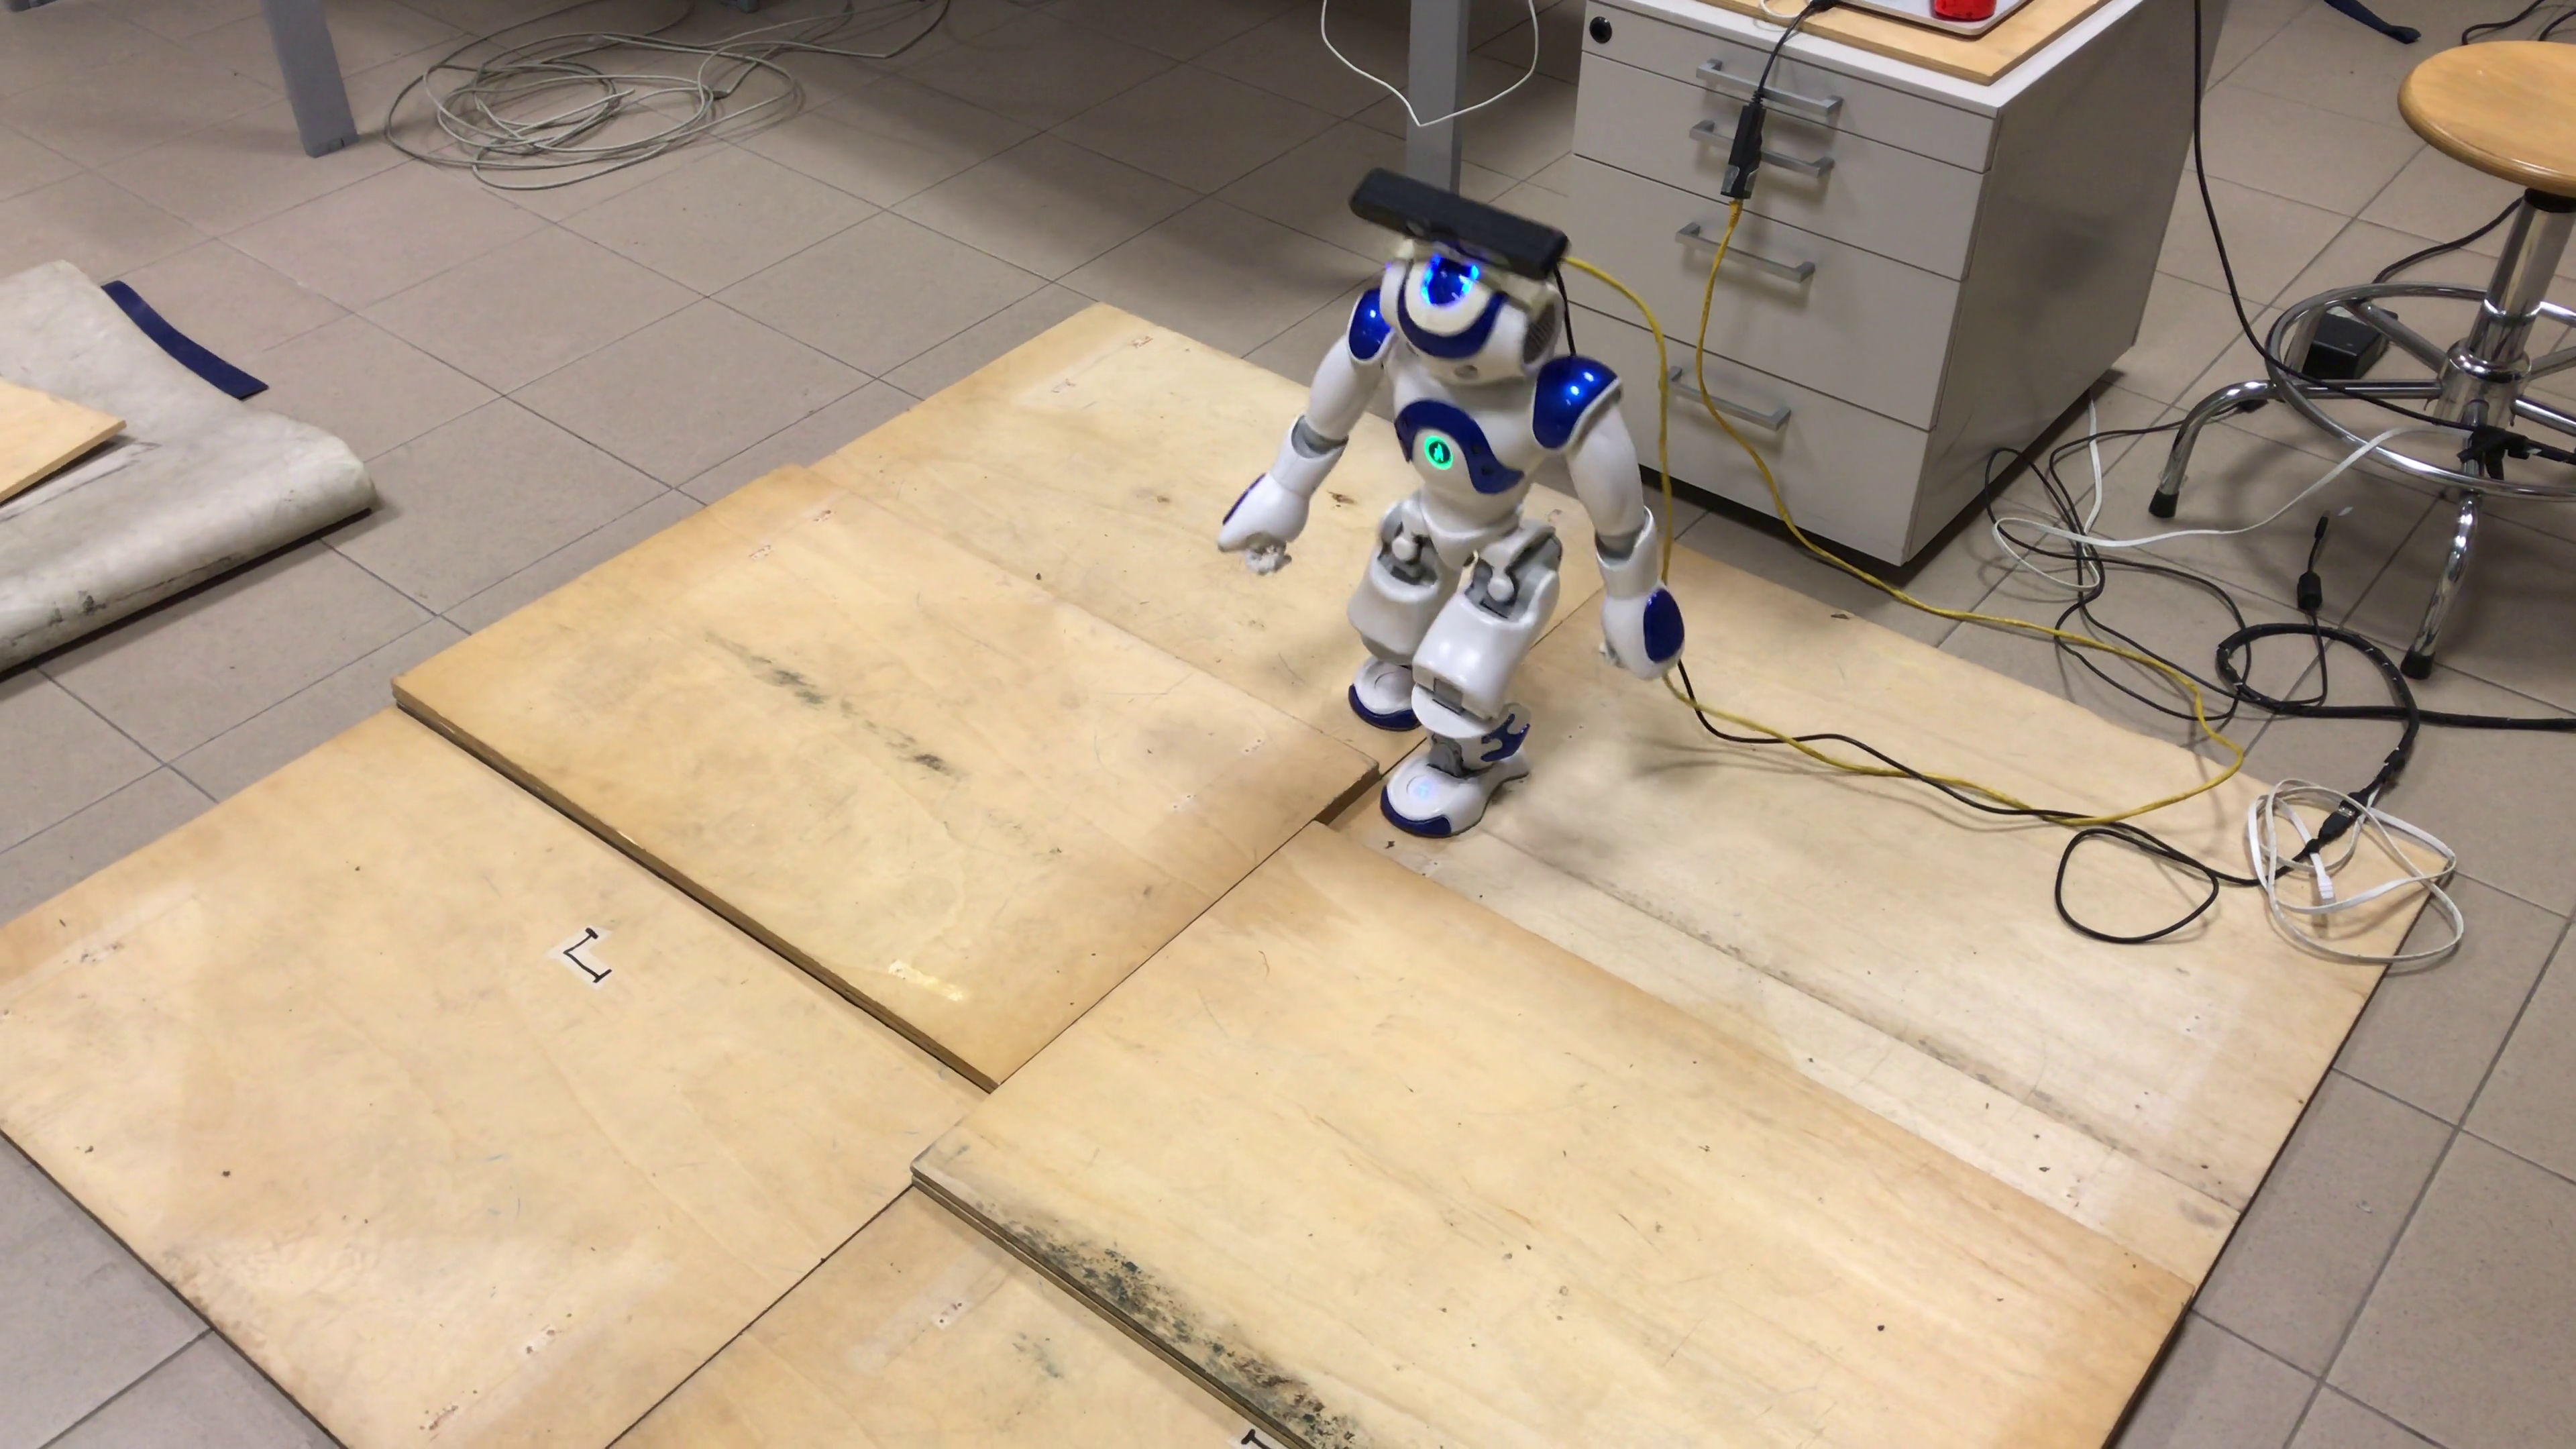
\includegraphics[width=\linewidth]
      {figures/experiments/unknown-env/video/04.png}
    \caption{Third step}
  \end{subfigure}
  \begin{subfigure}{0.48\textwidth}
    \includegraphics[width=\linewidth]
      {figures/experiments/unknown-env/video/05.png}
    \caption{Fourth step}
  \end{subfigure}\hspace*{\fill}
  \begin{subfigure}{0.48\textwidth}
    \includegraphics[width=\linewidth]
      {figures/experiments/unknown-env/video/06.png}
    \caption{Fifth step}
  \end{subfigure}
  \begin{subfigure}{0.48\textwidth}
    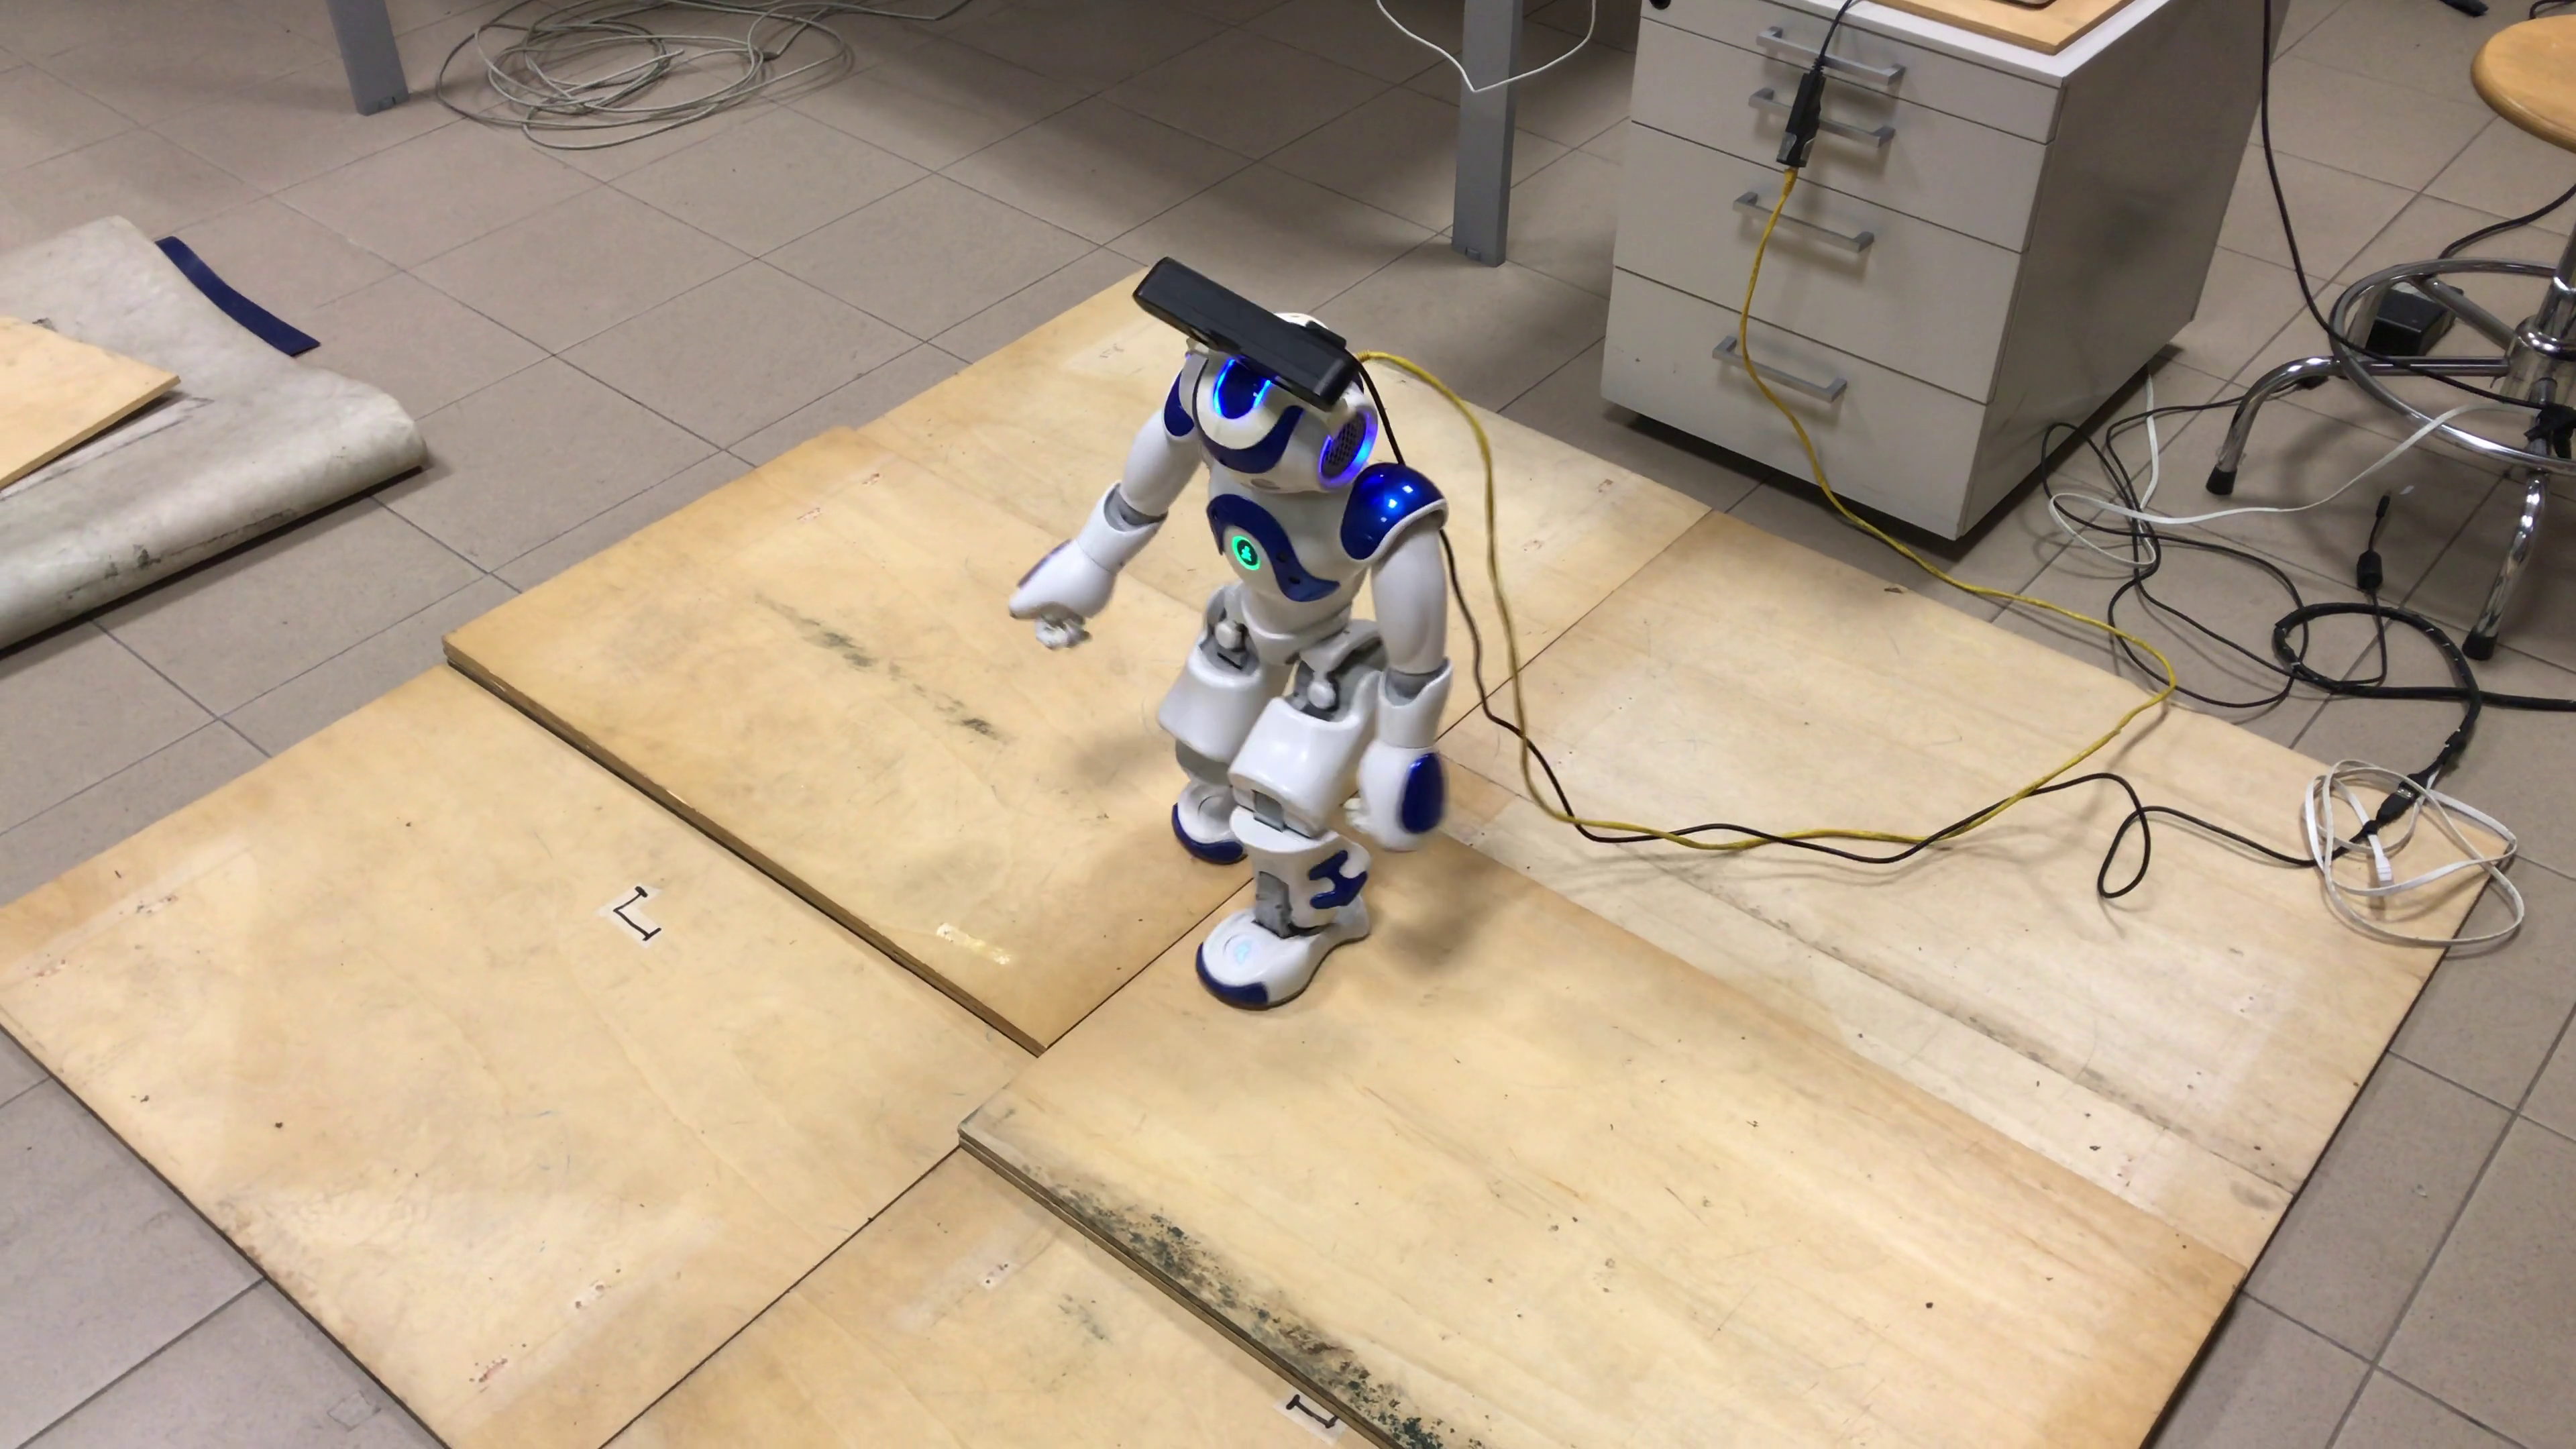
\includegraphics[width=\linewidth]
      {figures/experiments/unknown-env/video/07.png}
    \caption{Seventh step}
  \end{subfigure}\hspace*{\fill}
  \begin{subfigure}{0.48\textwidth}
    \includegraphics[width=\linewidth]
      {figures/experiments/unknown-env/video/08.png}
    \caption{Eighth step}
  \end{subfigure} \caption{The figures show the motion of the robot
      for the scenario ``Stair Climbing (Unknown Environment)''.
      The robot starts at 20 cm 
      from the first staircase (Fig. \ref{fig:exp:unkenv:frame1}). Before 
      starting the motion (Fig. \ref{fig:exp:unkenv:frame2}), an
      elevation map is built by the \texttt{elevation\_mapping} framework
      (Chapter \ref{ch:elevation-map-generation}),
      which receives the depth frames from the ASUS Xtion Pro placed 
      on top of the robot. The elevation map is sent to the planner, which 
      generates a footstep plan (Chapter \ref{ch:rrt-based-footstep-planning}).
      The footstep plan is then sent to the 
      robot, which executes the motion by using the Variable Height CoM
      IS-MPC (Chapter \ref{ch:vh-com-is-mpc}). The robot correctly manages to 
      climb the stairs without colliding with the staircases. Each staircase 
      has a height of 2 cm.}
  \label{fig:experiments:unkenv:videoframes}
\end{figure}

\begin{figure}
    \centering
    \includegraphics[width=0.95\textwidth]
        {figures/experiments/unknown-env/footstep-plan.pdf}
    \caption{Footstep plan generated for the scenario ``Stair Climbing in 
        Unknown Environments''.}
    \label{fig:experiments:unknown-env:footstep-plan}
\end{figure}
\begin{figure}
    \centering
    \includegraphics[width=0.95\textwidth]
        {figures/experiments/unknown-env/rrt-tree.pdf}
    \caption{Tree generated for the scenario ``Stair Climbing in 
        Unknown Environments''.}
    \label{fig:experiments:unknown-env:rrt-tree}
\end{figure}


\chapter{Conclusion}
\label{ch:conclusion}
\section{Results}
Brief recap of the work and recaps.

\section{Future Works}
What's next: tracker -> makes it possible to continuously build the map with 
elevation\_mapping -> replanning -> makes it possible to move in whatever 
environment (World of Stairs).

Rough environments?



\backmatter
% bibliography
\cleardoublepage
\phantomsection
%\bibliographystyle{sapthesis} % BibTeX style
\bibliographystyle{unsrt}
\bibliography{bibliography} % BibTeX database without .bib extension

\end{document}
